\documentclass{amsart}
 
%\linespread{2}

% PACKAGES ~~~~~~~~~~~~~~~~~~~~

\usepackage{amsfonts}
\usepackage{amssymb}  
\usepackage{amsthm} 
\usepackage{amsmath} 
\usepackage{caption}
\usepackage[inline]{enumitem}
\setlist{itemsep=0em, topsep=0em, parsep=0em}
\setlist[enumerate]{label=(\alph*)}
\usepackage{etoolbox}
\usepackage{stmaryrd} 
\usepackage[dvipsnames]{xcolor}

\definecolor{myurlcolor}{rgb}{0.6,0,0}
\definecolor{mycitecolor}{rgb}{0,0,0.8}
\definecolor{myrefcolor}{rgb}{0,0,0.8}
\usepackage[pagebackref]{hyperref}
\usepackage{hyperref}
\hypersetup{colorlinks,
	linkcolor=myrefcolor,
	citecolor=mycitecolor,
	urlcolor=myurlcolor}
\renewcommand*{\backref}[1]{(Referred to on page #1.)}

\usepackage{graphicx}
\graphicspath{ {img/} }
\usepackage{mathtools}

\usepackage{tikz}
\usetikzlibrary{matrix,arrows,shapes,decorations.markings,decorations.pathreplacing}
\usepackage{todonotes}

% NEW COMMANDS ~~~~~~~~~~~~~~~~~~

% symbols
\renewcommand{\epsilon}{\varepsilon}
\newcommand{\op}{^{\scriptsize{ \textrm{op} } }}
\newcommand{\iso}{\cong}
\renewcommand{\equiv}{\simeq}
\renewcommand{\hat}[1]{\widehat{#1}}

% categories
\newcommand{\A}{\cat{A}}
\newcommand{\B}{\cat{B}}
\newcommand{\C}{\cat{C}}
\newcommand{\D}{\cat{D}}
\newcommand{\E}{\cat{E}}
\renewcommand{\P}{\cat{P}}
\newcommand{\Q}{\cat{Q}}
\newcommand{\R}{\cat{R}}
\newcommand{\T}{\cat{T}}
\newcommand{\U}{\cat{U}}
\newcommand{\V}{\cat{V}}
\newcommand{\W}{\cat{W}}
\newcommand{\X}{\cat{X}}
\newcommand{\Y}{\cat{Y}}
\newcommand{\Z}{\cat{Z}}
\renewcommand{\AA}{\bicat{A}}
\newcommand{\BB}{\bicat{B}}
\newcommand{\CC}{\bicat{C}}
\newcommand{\DD}{\bicat{D}}
\newcommand{\EE}{\bicat{E}}
\newcommand{\PP}{\bicat{P}}
\newcommand{\QQ}{\bicat{Q}}
\newcommand{\RR}{\bicat{R}}
\newcommand{\TT}{\bicat{T}}
\newcommand{\UU}{\bicat{U}}
\newcommand{\VV}{\bicat{V}}
\newcommand{\WW}{\bicat{W}}
\newcommand{\XX}{\bicat{X}}
\newcommand{\YY}{\bicat{Y}}
\newcommand{\ZZ}{\bicat{Z}}
\newcommand{\AAA}{\dblcat{A}}
\newcommand{\BBB}{\dblcat{B}}
\newcommand{\CCC}{\dblcat{C}}
\newcommand{\DDD}{\dblcat{D}}
\newcommand{\EEE}{\dblcat{E}}
\newcommand{\MMM}{\dblecat{M}}
\newcommand{\PPP}{\dblcat{P}}
\newcommand{\QQQ}{\dblcat{Q}}
\newcommand{\RRR}{\dblcat{R}}
\newcommand{\SSS}{\dblcat{S}}
\newcommand{\TTT}{\dblcat{T}}
\newcommand{\UUU}{\dblcat{U}}
\newcommand{\VVV}{\dblcat{V}}
\newcommand{\WWW}{\dblcat{W}}
\newcommand{\XXX}{\dblcat{X}}
\newcommand{\YYY}{\dblcat{Y}}
\newcommand{\ZZZ}{\dblcat{Z}}

\newcommand{\Set}{\cat{Set}}
\newcommand{\Rel}{\cat{Rel}}
\newcommand{\Pos}{\cat{Pos}}
\newcommand{\Graph}{\cat{Graph}}
\newcommand{\RGraph}{\cat{RGraph}}
\newcommand{\Top}{\cat{Top}}
\newcommand{\Cat}{\cat{Cat}}
\newcommand{\Bicat}{\cat{Bicat}}
\newcommand{\DblCat}{\cat{DblCat}}
\newcommand{\Topos}{\cat{Topos}}
\newcommand{\Span}{\cat{Span}}
\newcommand{\Csp}{\cat{Csp}}
\newcommand{\Gram}{\cat{Gram}}
\newcommand{\StrCsp}{\cat{StrCsp}}
\newcommand{\SSStrCsp}{\dblcat{C} \textrm{sp}}
\newcommand{\StrCspGram}{\cat{StrCspGram}}
\newcommand{\MonSpCsp}{\dblcat{M} \textrm{onSpCsp}}

% functors
\newcommand{\core}{\mathbf{core}}
\newcommand{\Lang}{\mathrm{Lang}}

% text formatting
\newcommand{\defn}[1]{\textbf{#1}}
\newcommand{\cat}[1]{\mathsf{#1}}
\newcommand{\bicat}[1]{\mathbf{#1}}
\newcommand{\dblcat}[1]{\mathbb{#1}}
\newcommand{\type}[1]{\mathtt{#1}}
\newcommand{\edit}[1]{\textcolor{editcolour}{(#1)}}

% arrows
\newcommand{\from}{\colon}
\newcommand{\rel}{\nrightarrow}
\newcommand{\To}{\Rightarrow}
\newcommand{\xto}[1]{\xrightarrow{#1}}
\newcommand{\monicto}{\rightarrowtail}
\newcommand{\dderiv}[2]{#1 \rightsquigarrow #2}
\newcommand{\deriv}[2]{#1 \rightsquigarrow^\ast #2}
\renewcommand{\gets}{\leftarrow}
\newcommand{\monicgets}{\leftarrowtail}
\newcommand{\xgets}[1]{\xleftarrow{#1}}
\newcommand{\spn}[3]{#2 \to #1 \times #3}
\newcommand{\tospan}{\xrightarrow{\mathit{sp}}}
\newcommand{\csp}[3]{#1 + #3 \to #2}
\newcommand{\tocospan}{\xrightarrow{\mathit{csp}}}

% OPERATORS ~~~~~~~~~~~~~~~~~~

\DeclareMathOperator{\Hom}{Hom}
\DeclareMathOperator{\id}{id}
\DeclareMathOperator{\im}{im}
\DeclareMathOperator{\Sub}{Sub}
\DeclareMathOperator{\colim}{colim}

% ENVIRONMENTS & COUNTERS ~~~~~~~~~~~

\newtheorem{theorem}{Theorem}[section]
\newtheorem*{theorem*}{Theorem}
\newtheorem{lemma}[theorem]{Lemma}
\newtheorem{proposition}[theorem]{Proposition}
\newtheorem{corollary}[theorem]{Corollary}

\theoremstyle{remark}
\newtheorem{remark}[theorem]{Remark}
\newtheorem{notation}[theorem]{Notation}

\theoremstyle{definition}
\newtheorem{example}[theorem]{Example} 
\newtheorem{definition}[theorem]{Definition}

\setcounter{tocdepth}{1} % Sets depth for table of contents. 

% TIKZ TYPES ~~~~~~~~~~~~~~~~~~~~~

% arrow head in middle of edge
\tikzset{->-/.style={decoration={%
      markings,
      mark=at position .5 with {\arrow{>}}},postaction={decorate}}
}

% arrow head user-positioned
\tikzset{->-pos/.style={decoration={%
      markings,
      mark=at position #1 with {\arrow{>}}},postaction={decorate}}
}

% arrow head in middle of edge
\tikzset{-|->/.style={decoration={%
      markings,
      mark=at position .5 with {\arrow{|}},mark=at position 1 with {\arrow{>}}},postaction={decorate}}
}

% INLINE DIAGRAMS ~~~~~~~~~~~~~~~

% walking reflexive graph
\newcommand{\rgraph}[2]{%
  \begin{tikzpicture}[scale=0.75,baseline=-3pt]
    \node (a) at (0,0) {$ #1 $};
    \node (b) at (1,0) {$ #2 $};
    \draw [->]
    ([yshift= 4pt]a.east) to ([yshift= 4pt]b.west);
    \draw [->]
    ([yshift=-4pt]a.east) to ([yshift=-4pt]b.west);
    \draw [->]
    (b.west) to (a.east);
  \end{tikzpicture}
}

% walking graph
\newcommand{\graph}[2]{%
  \begin{tikzpicture}[scale=0.75,baseline=-3pt]
    \node (a) at (0,0) {$ #1 $};
    \node (b) at (1,0) {$ #2 $};
    \draw [->]
    ([yshift=4pt]a.east) to ([yshift=4pt]b.west);
    \draw [->]
    ([yshift=-4pt]a.east) to ([yshift=-4pt]b.west);
  \end{tikzpicture}
}

% open tipped arrow
\newcommand{\opento}[2]{%
  \begin{tikzpicture}[scale=0.75,baseline=-3pt]
    \node (a) at (0,0) {$ #1 $};
    \node (b) at (1,0) {$ #2 $};
    \draw [->, open triangle 60]
    (a.east) to (b.west);
  \end{tikzpicture}
}

% inline horizontal arrow
\newlength\mylen
\settowidth\mylen{$\to$}

\newcommand{\horarrow}{%
  \to\kern-0.55\mylen\vline height 1.2ex depth
  -0.4pt\kern0.55\mylen}

% adjunction
\newcommand{\adjunction}[4]{%
  \begin{tikzpicture}[baseline=-3pt]
    \node (1) at (0,0) {\( #1 \)};
    \node (2) at (2,0) {\( #4 \)};
    \draw [->]
    ([yshift= 4pt]2.west) to
    node [above] {\scriptsize{ $ #2 $ }}
    ([yshift= 4pt]1.east);
    \draw [->]
    ([yshift= -4pt]1.east) to
    node [below] {\scriptsize{ $ #3 $ }}
    node [above,yshift= -1.5pt] {\scriptsize{$ \perp $}}
    ([yshift= -4pt]2.west);
  \end{tikzpicture}
  % 
}

% ~~~~~~~~~~~~~~~~~~~~~~~~~~~~~~~~~~~~~~~~
% 
% ~~~~~~~~~~~ begin document~~~~~~~~~~~~~~
% 
% ~~~~~~~~~~~~~~~~~~~~~~~~~~~~~~~~~~~~~~~~

\begin{document}

\author{Daniel Cicala}
\title{Rewriting structured cospans}
\date{\today}
\email{cicala@math.ucr.edu}
\address{Department of Mathematics\\
  University of California, Riverside\\
  Riverside, California 92521}
\maketitle

\begin{abstract}
  To foster the study of networks on an abstract level, we
  further study the formalism of \emph{structured cospans}
  introduced by Baez and Courser. A structured cospan is a
  diagram of the form $ La \to x \gets Lb $ built from a
  geometric morphism with left exact left adjoint
  $ L \dashv R \from \X \to \A $.  We show that this
  construction is functorial and results in a topos with
  structured cospans for objects.  Additionally, structured
  cospans themselves are compositional. Combining these two
  perspectives, we define a double category of structured
  cospans.  We then leverage adhesive categories to create a
  theory of rewriting for structured cospans. We generalize
  the result from graph rewriting stating that a graph
  grammar induces the same rewrite relation as its
  underlying graph grammar.  We use this fact to prove our
  main result, a complete characterization of the rewriting
  relation for a topos $ \X $ using double categories.  This
  provides a compositional framework for rewriting systems.
\end{abstract}

% ~~~~~~~~~~~~~~~~~~~~~~~~~~~~~~~~~~~~~~~~
% ~~~~~~~~~~~ introduction ~~~~~~~~~~~~~~~
% ~~~~~~~~~~~~~~~~~~~~~~~~~~~~~~~~~~~~~~~~

\section{Introduction}
\label{sec:Introduction}

This paper is part of a program that aims to study open
systems by treating them as morphisms in a category
\cite{PassiveNets,MrkvProc,RxNets,OpenPetri,Cic_SpCsp}. Baez
and Courser invented structured cospans, a syntactical
device to reason about open systems. In this paper, we
introduce a theory of rewriting to structured cospans.

In the study of formal languages, a rewriting system often
accompanies a syntax.  Roughly, a rewriting system is a set
of rules, each providing a way to rewrite one syntactical
term into another.  Each rewriting system gives rise to the
\emph{rewriting relation} that relates two terms if one can
be rewritten into the other using a finite sequence of
rules. This relates syntactical terms with the same meaning.
An example is when one replaces two resistors wired in
series with a single resistor with aggregate resistance.  An
appropriate rewriting system would want to relate (not
equate) these.

The theory of rewriting has gone through several epochs,
each more abstract from the last.  Noam Chomsky introduced rewriting for formal languages \cite{Chomsky}. Here, the
syntactical terms in consideration were strings of
characters, or letters.  Later, Ehrig,
et.\ al.\ \cite{Ehrig_GraphGram} used pushouts to introduce
rewriting for graphs.  Graph rewriting was then axiomatised
by Lack and Soboci\'{n}ski when they defined adhesive
categories \cite{LackSobo_Adhesive}.  While we do not need
the full generality of adhesive categories, we do use
rewriting of topoi, which are examples of adhesive
categories \cite{LackSobo_ToposIsAdh}.

Central to rewriting is the concept of a grammar, which we
define to be a topos $ \X $ paired with a set of rules
$ P $.  Each rule in $ P $ is a span
$ \ell \monicgets k \monicto r $ in $ \X $ with two monic
legs.  The idea is that $ r $ replaces $ \ell $ and the common subobject $ k $ remains fixed.  The
grammar $ ( \X , P ) $ induces a \emph{derived grammar}
$ ( \X , P' ) $ where the rules comprising $ P' $ 
appear on the bottom row of a double pushout diagram of
form
% 
\[
  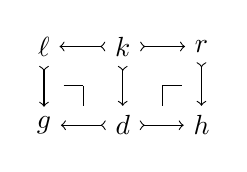
\begin{tikzpicture}
    \node (1) at (0,1) {$ \ell $};
    \node (2) at (1,1) {$ k $};
    \node (3) at (2,1) {$ r $};
    \node (4) at (0,0) {$ g $};
    \node (5) at (1,0) {$ d $};
    \node (6) at (2,0) {$ h $};
    \draw [>->] (2) to node [] {\scriptsize{$  $}} (1);
    \draw [>->] (2) to node [] {\scriptsize{$  $}} (3);
    \draw [>->] (5) to node [] {\scriptsize{$  $}} (4);
    \draw [>->] (5) to node [] {\scriptsize{$  $}} (6);
    \draw [>->] (1) to node [] {\scriptsize{$  $}} (4);
    \draw [>->] (2) to node [] {\scriptsize{$  $}} (5);
    \draw [>->] (3) to node [] {\scriptsize{$  $}} (6);
    % corners
    \begin{scope}[shift={(0,0)}]
      % \draw [-] (0,0) to (0,0.25);
      \draw [-] (0.25,0.5) to node [] {} (0.5,0.5);
      \draw [-] (0.5,0.5) to node [] {} (0.5,0.25);
    \end{scope}
    % corners
    \begin{scope}[shift={(1.5,0)}]
      \draw [-] (0,0.25) to (0,0.5);
      \draw [-] (0,0.5) to node [] {} (0.25,0.5);
      % \draw [-] (0.25,0.25) to node [] {} (0.25,0);
    \end{scope}
  \end{tikzpicture}
\]
%
whose top row belongs to $ P $. To study the grammar
$ ( \X , P ) $, we try to understand the \emph{rewrite
  relation} $ \deriv{g}{h} $ defined by, first, relating
objects if there is a rule in $ P' $ between them, then
taking the reflexive and transitive closure.

In practice, we take $ \X $ to be a topos which thought of as systems together with appropriate morphisms.  Our favorite example is the category $ \RGraph $
of reflexive graphs. We like graphs because of their
importance in network theory. We like reflexive graphs because the terminal object represents the nodes.  Given a
grammar $ ( \X , P ) $, our goal is to rewrite systems $ x $
by decomposing it into subsystems, rewriting those, then
connecting the results back together.  Using structured
cospans, we do this in a way that characterizes the
rewriting relation for $ ( \X , P ) $.

To do this, we turn to Gadducci and Heckle
\cite{Gadd_IndGraphTrans}, who introduced an inductive
perspective for graph rewriting. This mirrors our present goals so we follow the framework set in their
paper.  They define so called ``ranked graphs'' which are
directed graphs with an interface, that is two sets of
nodes, one set containing \emph{input nodes} and the other
containing \emph{output nodes}. Using structured cospans,
we are able to provide inputs and outputs to a much wider
class of objects than graphs.

We make note that the terms 'input' and 'output' are not
meant to imply causal structure.

To start, we need data beyond a topos $ \X $.
We begin with a geometric morphism
%
\[
  ( L \from \A \to \X ) \dashv ( R \from \X \to \A ),
\]
% 
which, recall, is an adjunction between topoi whose left
adjoint preserves finite limits.  In this setup, $ \X $ is
still our topos of systems and $ \A $ is a topos comprised
of ``interface types''.  These serve as the boundaries along
which we decompose the systems in $ \X $.  The left adjoint
$ L $ serves as the channel through which we port the
interface types into $ \X $ so that they can interact with
the systems.  The properties of a geometric morphism arise
throughout this article.

Given a geometric morphism $ L \dashv R $, a
\emph{structured cospan} is a diagram in $ \X $ of the form
$ La \to x \gets Lb $. Think of this as consisting of a system $ x $ with inputs $ a $ and outputs $ b $.

Baez and Courser introduced structured cospans
\cite{StrCsp}, though to introduce rewriting, we need
stronger hypotheses.  They focused primary on the
compositional structure, which the describe as follows. A
structured cospan $ La \to x \gets Lb $ with outputs $ b $
can connect with a structured cospan $ Lb \to y \gets Lc $
with inputs $ b $ via pushout
%
\[
  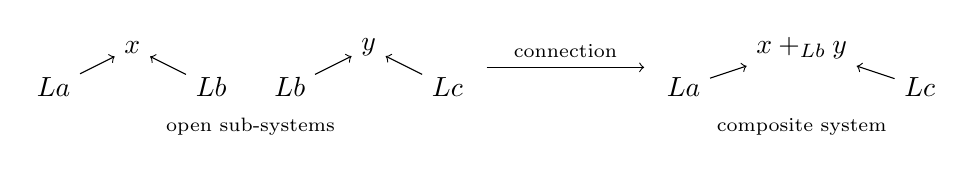
\begin{tikzpicture}
    \begin{scope}
      \node (1) at (0,0) {$ La $};
      \node (2) at (1,0.5) {$ x $};
      \node (3) at (2,0) {$ Lb $};
      \node (4) at (3,0) {$ Lb $};
      \node (5) at (4,0.5) {$ y $};
      \node (6) at (5,0) {$ Lc $};
      \draw [->] (1) to node [] {\scriptsize{$  $}} (2);
      \draw [->] (3) to node [] {\scriptsize{$  $}} (2);
      \draw [->] (4) to node [] {\scriptsize{$  $}} (5);
      \draw [->] (6) to node [] {\scriptsize{$  $}} (5);
      \node () at (2.5,-0.5) {\scriptsize{open sub-systems}};
    \end{scope}
    %
    \begin{scope}[shift={(8,0)}]
      \node (1) at (0,0) {$ La $};
      \node (2) at (1.5,0.5) {$ x +_{Lb} y $};
      \node (3) at (3,0) {$ Lc $};
      \draw [->] (1) to node [] {\scriptsize{$  $}} (2);
      \draw [->] (3) to node [] {\scriptsize{$  $}} (2);
      \node () at (1.5,-0.5) {\scriptsize{composite system}};
    \end{scope}
    %
    \draw [->] (5.5,0.25) to node [above] {\scriptsize{connection}} (7.5,0.25);    
  \end{tikzpicture}
\]
% 
This gives us a category $ _{L}\Csp $ whose objects are from
$ \A $ and whose arrows are the structured cospans.

Observe that a system $ x $ with an empty interface can be
encoded using the structured cospan $ L0 \to x \gets L0 $.
A local view of $ x $ is a decomposition
%
\[
  L0 \to x_1 \gets Lb_1 \to x_2 \gets Lb_2 \dotsm Lb_{n-1} \to x_n
  \gets L0
\]
% 
and individually looking at each factor.
    
To study the rewriting of a system with interface,
we can introduce a category where structured cospans are
objects. Morphisms of structured cospans are commuting diagrams
%
\begin{equation} \label{eq:StrCsp-arrows}
\raisebox{-4.5ex}{
  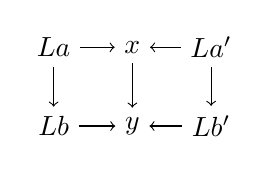
\begin{tikzpicture}
    \node (1t) at (0,1) {$ La $};
    \node (2t) at (1,1) {$ x $};
    \node (3t) at (2,1) {$ La' $};
    \node (1b) at (0,0) {$ Lb $};
    \node (2b) at (1,0) {$ y $};
    \node (3b) at (2,0) {$ Lb' $};
    \draw [->] (1t) to node [] {\scriptsize{$  $}} (2t);
    \draw [->] (3t) to node [] {\scriptsize{$  $}} (2t);
    \draw [->] (1b) to node [] {\scriptsize{$  $}} (2b);
    \draw [->] (3b) to node [] {\scriptsize{$  $}} (2b);
    \draw [->] (1t) to node [] {\scriptsize{$  $}} (1b);
    \draw [->] (2t) to node [] {\scriptsize{$  $}} (2b);
    \draw [->] (3t) to node [] {\scriptsize{$  $}} (3b);
  \end{tikzpicture}
}
\end{equation}
%
Structured cospans and their arrows form a category
$ _{L}\StrCsp $.  Our first result is about this category.

\begin{theorem*}[\ref{thm:strcsp-istopos}]
  $ _{L}\StrCsp $ is a topos.
\end{theorem*}

This theorem allows us to introduce rewriting systems into
structured cospans.  As mentioned above, the rewriting
system starts with grammars, though we restrict our
attention to \emph{structured cospan grammar}.  This is a
grammar $ ( _{L}\StrCsp , P ) $ where $ P $ has rules of the
form
%
 \[
   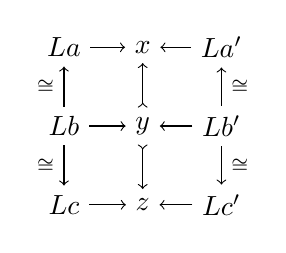
\begin{tikzpicture}
    \begin{scope}
        \node (1) at (0,2) {\( La \)};
        \node (2) at (1,2) {\( x \)};
        \node (3) at (2,2) {\( La' \)};
        \node (4) at (0,1) {\( Lb \)};
        \node (5) at (1,1) {\( y \)};
        \node (6) at (2,1) {\( Lb' \)};
        \node (7) at (0,0) {\( Lc \)};
        \node (8) at (1,0) {\( z \)};
        \node (9) at (2,0) {\( Lc' \)};
        \draw [->] (1) to node []
          {\scriptsize{\( \)}} (2);
        \draw [->] (3) to node []
          {\scriptsize{\( \)}} (2);
        \draw [->] (4) to node []
          {\scriptsize{\( \)}} (5);
        \draw [->] (6) to node []
          {\scriptsize{\( \)}} (5);
        \draw [->] (7) to node []
          {\scriptsize{\( \)}} (8);
        \draw [->] (9) to node []
          {\scriptsize{\( \)}} (8);
        \draw [->] (4) to node [left]
          {\scriptsize{\( \iso \)}} (1);
        \draw [->] (4) to node [left]
          {\scriptsize{\( \iso \)}} (7);
        \draw [>->] (5) to node []
          {\scriptsize{\( \)}} (2);
        \draw [>->] (5) to node []
          {\scriptsize{\( \)}} (8);
        \draw [->] (6) to node [right]
          {\scriptsize{\( \iso \)}} (3);
        \draw [->] (6) to node [right]
          {\scriptsize{\( \iso \)}} (9);
    \end{scope}
  \end{tikzpicture}
\]
%
As before, we associate to $ ( _{L}\StrCsp , P ) $ the
derived grammar $ ( _{L}\StrCsp , P' ) $ where $ P' $ is the
set of rules derived from the rules in $ P $ using the
double pushout approach.  In fact, this association is
functorial.  We define another functor assigning a double
category to $ ( _{L}\StrCsp , P' ) $ whose objects are from
$ \A $, vertical arrows are spans in $ \A $ with invertible
legs, horizontal arrows are structured cospans in
$ _{L}\StrCsp $, and whose squares are generated by the
rules in $ P' $. The \emph{language functor} is composite
$ \Lang $.  As we see below, $ \Lang $ encodes a rewriting
relation on $ \X $ inside the double category
$ \Lang ( _{L}\StrCsp , P ) $.

Using a double category allows us to combine into a single
structure the composability (horizontal composition) and
rewritability (vertical composition) of structured cospans.
The fact that this actually is a double category
\cite[Lem.~4.2]{CicCour_SpCspTopos} provides the interchange
law, which ensures the compatibility of composing and
rewriting systems. This compatibility grants us the ability
to decompose a system into subsystems, rewrite those, then
connect the results.

At this point, we begin to connect the rewriting relation on
a grammar $ ( \X , P ) $ with the language of a certain
structured cospan grammar $ ( _{L}\StrCsp , \hat{P} )
$. Here, our work begins to mirror that of Gadducci and
Heckle.  They use a well-known fact. Consider the sets
$ \{ \ell \monicgets k \monicto r \} $ and
$ \{ \ell \monicgets k_\flat \monicto r \} $ where
$ k_\flat $ is the discrete graph underlying $ k $.  These
each have the same rewrite relation
\cite[Prop.~3.3]{Ehrig_GraphGram}.

We prove a generalized version of this result. To understand
the following statement, denote by $ P_\flat $ the set of
rules obtained from
$ P = \{ \ell \monicgets k \monicto r \} $ by restricting
the the span legs along the counit $ LRk \to k $ of the
comonad $ LR $.

\begin{theorem*}[\ref{thm:production-same-rewrite-relation-as-discrete}]
  Fix a geometric morphism $ L \dashv R \from \X \to \A $
  with monic counit. Let $ ( \X , P ) $ be a grammar such
  that for every $ \X $-object $ x $ in the apex of a
  production of $ P $, the Heyting algebra $ \Sub (x) $ is
  well-founded.  The rewriting relation for a grammar
  $ ( \X , P ) $ is equal to rewriting relation for the
  grammar $ ( \X , P_{\flat} ) $.
\end{theorem*}

It follows from this theorem that we can study the rewriting
relation for $ ( \X , P_\flat ) $ instead of the rewriting
relation for $ ( \X , P ) $.

Now, to decompose the systems in $ \X $ and the rules in
$ P $, we associate to $ ( \X , P ) $ the structured cospan
grammar $ ( _{L}\StrCsp , \hat{P} ) $ where $ \hat{P} $
contains
%
\[
  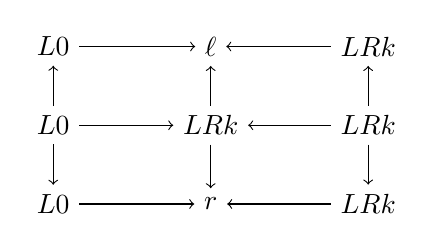
\begin{tikzpicture}
    \node (1) at (0,2) {$ L 0 $};
    \node (2) at (2,2) {$ \ell $};
    \node (3) at (4,2) {$ LRk $};
    \node (4) at (0,1) {$ L 0 $};
    \node (5) at (2,1) {$ LRk $};
    \node (6) at (4,1) {$ LRk $};
    \node (7) at (0,0) {$ L 0 $};
    \node (8) at (2,0) {$ r $};
    \node (9) at (4,0) {$ LRk $};
    \draw [->] (1) to node [] {\scriptsize{$  $}} (2);
    \draw [->] (3) to node [] {\scriptsize{$  $}} (2);
    \draw [->] (4) to node [] {\scriptsize{$  $}} (5);
    \draw [->] (6) to node [] {\scriptsize{$  $}} (5);
    \draw [->] (7) to node [] {\scriptsize{$  $}} (8);
    \draw [->] (9) to node [] {\scriptsize{$  $}} (8);
    \draw [->] (4) to node [] {\scriptsize{$  $}} (1);
    \draw [->] (4) to node [] {\scriptsize{$  $}} (7);
    \draw [->] (5) to node [] {\scriptsize{$  $}} (2);
    \draw [->] (5) to node [] {\scriptsize{$  $}} (8);
    \draw [->] (6) to node [] {\scriptsize{$  $}} (3);
    \draw [->] (6) to node [] {\scriptsize{$  $}} (9);
  \end{tikzpicture}
\]
% 
for every rule $ LRk \to \ell \times r $ of $ P_{\flat} $.

This structured cospan grammar turns a system
$ x $ in $ \X $ into a structured cospan
$ L0 \to x \gets L0 $ with an empty interface and turns
the rules from $ P $ into what we can think of as generators
$ \hat{P} $ for a double category.  The main result of the
paper is that the rewriting relation for $ ( \X,P ) $ is
encoded inside a vertical hom-set of a double category
generated by structured cospans.

\begin{theorem*}[\ref{thm:inductive-rewriting}]
  Fix a geometric morphism $ L \dashv R \from \X \to \A $
  with monic counit. Let $ ( \X , P ) $ be a grammar such
  that for every $ \X $-object $ x $ in the apex of a
  production of $ P $, the Heyting algebra $ \Sub (x) $ is
  well-founded. Given $ g $, $ h \in \X $, then
  $ \deriv{g}{h} $ in the rewriting relation for a grammar
  $ ( \X , P ) $ if and only if there is a square
  %
  \[
    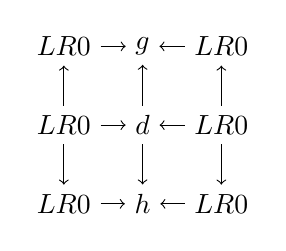
\begin{tikzpicture}
      \node (1t) at (0,2) {$ LR 0 $};
      \node (2t) at (1,2) {$ g $};
      \node (3t) at (2,2) {$ LR 0 $};
      \node (1m) at (0,1) {$ LR 0 $};
      \node (2m) at (1,1) {$ d $};
      \node (3m) at (2,1) {$ LR 0 $};
      \node (1b) at (0,0) {$ LR 0 $};
      \node (2b) at (1,0) {$ h $};
      \node (3b) at (2,0) {$ LR 0 $};
      \draw [->] (1t) to node [] {\scriptsize{$  $}} (2t);
      \draw [->] (3t) to node [] {\scriptsize{$  $}} (2t);
      \draw [->] (1m) to node [] {\scriptsize{$  $}} (2m);
      \draw [->] (3m) to node [] {\scriptsize{$  $}} (2m);
      \draw [->] (1b) to node [] {\scriptsize{$  $}} (2b);
      \draw [->] (3b) to node [] {\scriptsize{$  $}} (2b);
      \draw [->] (1m) to node [] {\scriptsize{$  $}} (1t);
      \draw [->] (1m) to node [] {\scriptsize{$  $}} (1b);
      \draw [->] (2m) to node [] {\scriptsize{$  $}} (2t);
      \draw [->] (2m) to node [] {\scriptsize{$  $}} (2b);
      \draw [->] (3m) to node [] {\scriptsize{$  $}} (3t);
      \draw [->] (3m) to node [] {\scriptsize{$  $}} (3b);
    \end{tikzpicture}
  \]
  % 
  in the double category $ \Lang ( _{L}\StrCsp , \hat{P} ) $.
\end{theorem*}

This theorem characterizes the rewriting relation as squares
framed by $ 0 $ inside of a double category. Given any
decomposition of a system $ x $ into structured cospans
%
\[
  L0 \to x_1 \gets La_1 \to x_2 \gets La_2 \dotsm La_{n-1} \to x_n
  \gets L0
\]
%
we can rewrite each structured cospan using rewriting rules. This will give a pasting diagram of the
sort
% 
\[
  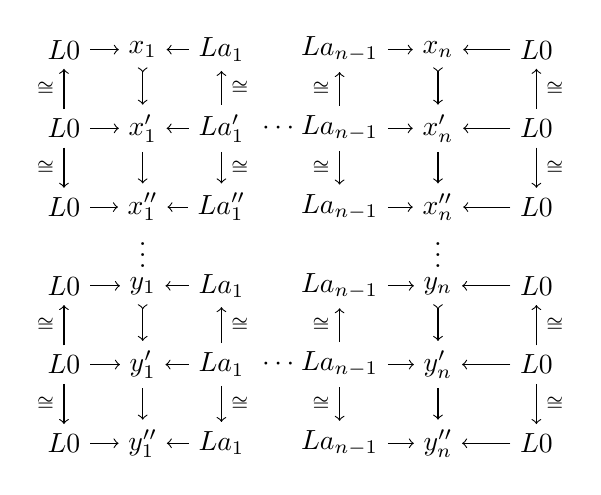
\begin{tikzpicture}
    \begin{scope}[shift={(0,3)}]
      \node (1) at (0,2) {$ L0 $};
      \node (2) at (1,2) {$ x_1 $};
      \node (3) at (2,2) {$ La_1 $};
      \node (4) at (0,1) {$ L0 $};
      \node (5) at (1,1) {$ x'_1 $};
      \node (6) at (2,1) {$ La'_1 $};
      \node (7) at (0,0) {$ L0 $};
      \node (8) at (1,0) {$ x''_1 $};
      \node (9) at (2,0) {$ La''_1 $};
      \draw [->] (1) to node [] {\scriptsize{$  $}} (2);
      \draw [->] (3) to node [] {\scriptsize{$  $}} (2);
      \draw [->] (4) to node [] {\scriptsize{$  $}} (5);
      \draw [->] (6) to node [] {\scriptsize{$  $}} (5);
      \draw [->] (7) to node [] {\scriptsize{$  $}} (8);
      \draw [->] (9) to node [] {\scriptsize{$  $}} (8);
      \draw [->] (4) to node [left] {\scriptsize{$ \cong $}} (1);
      \draw [->] (4) to node [left] {\scriptsize{$ \cong $}} (7);
      \draw [>->] (2) to node [] {\scriptsize{$  $}} (5);
      \draw [->] (5) to node [] {\scriptsize{$  $}} (8);
      \draw [->] (6) to node [right] {\scriptsize{$ \cong  $}} (3);
      \draw [->] (6) to node [right] {\scriptsize{$ \cong $}} (9);
    \end{scope}
    %
    \begin{scope}[shift={(3.5,3)}]
      \node (1) at (0,2) {$ La_{n-1} $};
      \node (2) at (1.25,2) {$ x_n $};
      \node (3) at (2.5,2) {$ L0 $};
      \node (4) at (0,1) {$ La_{n-1} $};
      \node (5) at (1.25,1) {$ x'_n $};
      \node (6) at (2.5,1) {$ L0 $};
      \node (7) at (0,0) {$ La_{n-1} $};
      \node (8) at (1.25,0) {$ x''_n $};
      \node (9) at (2.5,0) {$ L0 $};
       \draw [->] (1) to node [] {\scriptsize{$  $}} (2);
      \draw [->] (3) to node [] {\scriptsize{$  $}} (2);
      \draw [->] (4) to node [] {\scriptsize{$  $}} (5);
      \draw [->] (6) to node [] {\scriptsize{$  $}} (5);
      \draw [->] (7) to node [] {\scriptsize{$  $}} (8);
      \draw [->] (9) to node [] {\scriptsize{$  $}} (8);
      \draw [->] (4) to node [left] {\scriptsize{$ \cong $}} (1);
      \draw [->] (4) to node [left] {\scriptsize{$ \cong $}} (7);
      \draw [>->] (2) to node [] {\scriptsize{$  $}} (5);
      \draw [->] (5) to node [] {\scriptsize{$  $}} (8);
      \draw [->] (6) to node [right] {\scriptsize{$ \cong  $}} (3);
      \draw [->] (6) to node [right] {\scriptsize{$ \cong $}} (9);
    \end{scope}
    %
    \begin{scope}
      \node (1) at (0,2) {$ L0 $};
      \node (2) at (1,2) {$ y_1 $};
      \node (3) at (2,2) {$ La_1 $};
      \node (4) at (0,1) {$ L0 $};
      \node (5) at (1,1) {$ y'_1 $};
      \node (6) at (2,1) {$ La_1 $};
      \node (7) at (0,0) {$ L0 $};
      \node (8) at (1,0) {$ y''_1 $};
      \node (9) at (2,0) {$ La_1 $};
       \draw [->] (1) to node [] {\scriptsize{$  $}} (2);
      \draw [->] (3) to node [] {\scriptsize{$  $}} (2);
      \draw [->] (4) to node [] {\scriptsize{$  $}} (5);
      \draw [->] (6) to node [] {\scriptsize{$  $}} (5);
      \draw [->] (7) to node [] {\scriptsize{$  $}} (8);
      \draw [->] (9) to node [] {\scriptsize{$  $}} (8);
      \draw [->] (4) to node [left] {\scriptsize{$ \cong $}} (1);
      \draw [->] (4) to node [left] {\scriptsize{$ \cong $}} (7);
      \draw [>->] (2) to node [] {\scriptsize{$  $}} (5);
      \draw [->] (5) to node [] {\scriptsize{$  $}} (8);
      \draw [->] (6) to node [right] {\scriptsize{$ \cong  $}} (3);
      \draw [->] (6) to node [right] {\scriptsize{$ \cong $}} (9);
    \end{scope}
    %
    \begin{scope}[shift={(3.5,0)}]
      \node (1) at (0,2) {$ La_{n-1} $};
      \node (2) at (1.25,2) {$ y_n $};
      \node (3) at (2.5,2) {$ L0 $};
      \node (4) at (0,1) {$ La_{n-1} $};
      \node (5) at (1.25,1) {$ y'_n $};
      \node (6) at (2.5,1) {$ L0 $};
      \node (7) at (0,0) {$ La_{n-1} $};
      \node (8) at (1.25,0) {$y''_n $};
      \node (9) at (2.5,0) {$ L0 $};
       \draw [->] (1) to node [] {\scriptsize{$  $}} (2);
      \draw [->] (3) to node [] {\scriptsize{$  $}} (2);
      \draw [->] (4) to node [] {\scriptsize{$  $}} (5);
      \draw [->] (6) to node [] {\scriptsize{$  $}} (5);
      \draw [->] (7) to node [] {\scriptsize{$  $}} (8);
      \draw [->] (9) to node [] {\scriptsize{$  $}} (8);
      \draw [->] (4) to node [left] {\scriptsize{$ \cong $}} (1);
      \draw [->] (4) to node [left] {\scriptsize{$ \cong $}} (7);
      \draw [>->] (2) to node [] {\scriptsize{$  $}} (5);
      \draw [->] (5) to node [] {\scriptsize{$  $}} (8);
      \draw [->] (6) to node [right] {\scriptsize{$ \cong  $}} (3);
      \draw [->] (6) to node [right] {\scriptsize{$ \cong $}} (9);
    \end{scope}
    %
    \node () at (2.75,4) {$ \dotsm $};
    \node () at (1,2.5) {$ \vdots $};
    \node () at (2.75,1) {$ \dotsm $};
    \node () at (4.75,2.5) {$ \vdots $};
  \end{tikzpicture}
\]
%
Then we can compose these squares in any order to get a
rewriting on the original system $ x $ as desired.

The structure of this paper is as follows.  Section
\ref{sec:StrCsp} defines structured cospans and looks at the
perspective of these as objects and as arrows. Here,we give
our first main result: Theorem \ref{thm:strcsp-istopos}
which states that $ _{L}\StrCsp $ is a topos.  Section
\ref{sec:rewriting} consists of three parts.  The first is a
brief overview of double pushout rewriting as applied to
topoi.  The second part contains our second result, Theorem
\ref{thm:production-same-rewrite-relation-as-discrete} which
states that a grammar and its associated discrete grammar
have the same rewrite relation.  By the associated discrete
grammar, we mean that for each rule in the grammar, we are
restricting the apex $ k $ to its maximal interface, the
subobject $ LRk $.  The final part of this section contains
our main result, Theorem \ref{thm:inductive-rewriting}.

The author would like to thank John Baez and Fabio Gadducci
for helpful conversations.

% ~~~~~~~~~~~~~~~~~~~~~~~~~~~~~~~~~~~~~~~~
% ~~~~~~~~~~~ structured cospans~~~~~~~~~~
% ~~~~~~~~~~~~~~~~~~~~~~~~~~~~~~~~~~~~~~~~

\section{Structured Cospans}
\label{sec:StrCsp}

Baez and Courser introduced structured cospans to provide
syntax for compositional systems \cite{StrCsp}.  Because
structured cospans are a syntax, we want to set up a
framework that can reflect semantics. We propose double
pushout rewriting for this framework.

In this section, we set our hypotheses and explore
structured cospans in this context. In particular, we see
how, as morphisms, they encode compositional structure. We
also see them as objects of a topos. Using double
categories we combine the two perspectives.

Fix an adjunction
%
\[
  \adjunction{\X}{L}{R}{\A}
\]
%
between (elementary) topoi with $ L $ preserving finite
limits. Readers familiar with topos theory will recognize
this as a \emph{geometric morphism}. We use the notation
%
\(
  \langle f,g \rangle \from \spn{x}{y}{z}
\)
% 
for a span
%
\[
  x \xgets{f} y \xto{g} z
\]
%
and
%
\(
  [ f,g ] \from \csp{x}{y}{z}
\)
% 
for a cospan
%
\[
  x \xto{f} y \xgets{g} z.
\]
% 
Note that all categories in this paper have products and
coproducts, so this notation is safe to use.

% ~~~~~~~~~~~~~~~~~~~~~~~~
% ~~~~~~~~~~~~~~~~~~~~~~~~

\subsection{Structured cospans as arrows}
\label{sec:StrCsp-as-Arrows}

After defining structured cospans, we look at their
compositional structure. This material is in Baez
and Courser's work \cite{StrCsp}, but we include it here for
completeness.

\begin{definition}\label{df:strcsp}
  A \defn{structured cospan} is a cospan of the form
  $ \csp{La}{x}{Lb} $.  When we want to emphasize $ L $, we
  use the term $ L $-structured cospans.
\end{definition}

View $ \X $ as a category of closed systems and their
morphisms. By a \emph{closed system}, we mean a system that
cannot interact with the outside world. Think of $ \A $ as a
category of interfaces types and their morphisms. By
transporting the interface types along $ L $, they can be
combined with the systems in $ \X $.  A system is
\emph{open} when equipped with an interface.  Open systems
can interact with other compatible open systems.  Finally,
$ R $ returns the largest subobject of a system that can
serve as an interface.

Through this perspective, a structured cospan consists of a
closed system $ x $ equipped with the interface described by
the arrows from $ La $ and $ Lb $. Ignoring causality, we call $ La $ the input to $ x $ and
$ Lb $ the output. In fact, this convention is arbitrary because $ _{L}\Csp $ from
Definition \ref{def:strcsp-arr} is compact closed
\cite{CicCour_SpCspTopos}.

\begin{definition}
\label{def:strcsp-arr}  
Denote by $ _{L}\Csp $ the category that has the same
objects as $ \A $ and structured cospans $ \csp{La}{x}{Lb} $
as arrows of type $ a \to b $.
\end{definition}

Composing $ \csp{La}{x}{Lb} $ with $ \csp{Lb}{y}{Lc} $ uses
pushout
%
\[
  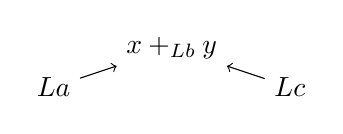
\begin{tikzpicture}
    \begin{scope}[]
    \node (1) at (0,0) {\( La \)};
    \node (2) at (1.5,0.5) {\( x +_{Lb} y \)};
    \node (3) at (3,0) {\( Lc \)};
     \draw [->] (1) to node [] {\scriptsize{\(  \)}} (2);
    \draw [->] (3) to node [] {\scriptsize{\(  \)}} (2); 
    \end{scope}
  \end{tikzpicture}
\]
% 
In a sense, pushouts glue objects together making it a
sensible way to model system connection.  The composition
above is like connecting along $ Lb $. We illustrate this
with open graphs. 

\begin{example}
\label{ex:open-graph-as-arrow}  
  Graph theory plays a central role in network theory.  As
  such we take open graphs to be primary example of a
  structured cospan. While this notion is not new
  \cite{DixKiss_OpenGraphs,Gadd_IndGraphTrans}, our
  infrastructure generalizes it.

  Denote by $ \RGraph $ the category of (directed reflexive
  multi-) graphs. There is a geometric morphism
  %
  \[
    \adjunction{\RGraph}{L}{R}{\Set}
  \]
  % 
  where $ Rx $ is the node set of graph $ x $ and $ La $ is
  the edgeless graph with node set $ a $. An \defn{open
    graph} is a cospan
  %
  \(
      \csp{La}{x}{Lb}
  \)
  % 
  for sets $ a $, $ b $, and graph $ x $. An illustrated
  example, with the reflexive loops suppressed, is
  %
  \[
    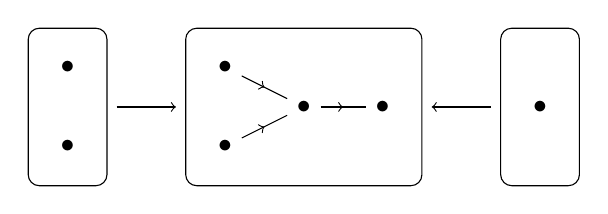
\begin{tikzpicture}
      %
      \begin{scope} % left graph
      \node (1) at (0,1) { \( \bullet \) };
      \node (2) at (0,0) { \( \bullet \) };
      \draw [rounded corners] (-0.5,-0.5) rectangle (0.5,1.5);
      \end{scope}
      %
      \begin{scope}[shift={(2,0)}] % center graph
      \node (1) at (0,1) {\( \bullet \)};
      \node (2) at (0,0) {\( \bullet \)};
      \node (3) at (1,0.5) {\( \bullet  \)};
      \node (4) at (2,0.5) {\( \bullet  \)};
      \draw [->-] (1) to (3);
      \draw [->-] (2) to (3);
      \draw [->-] (3) to (4);
      \draw [rounded corners] (-0.5,-0.5) rectangle (2.5,1.5);
      \end{scope}
      %
      \begin{scope}[shift={(6,0)}] % right graph
      \node (1) at (0,0.5) {\( \bullet \)};
      \draw [rounded corners] (-0.5,-0.5) rectangle (0.5,1.5);
      \end{scope}
      %
      \begin{scope} % graph morphisms
        \node (1) at (0.5,0.5) {};
        \node (2) at (1.5,0.5) {};
        \node (3) at (4.5,0.5) {};
        \node (4) at (5.5,0.5) {};
        \draw [->] (1) to (2);
        \draw [->] (4) to (3);
      \end{scope}
    \end{tikzpicture}
  \]
  % 
  The boxed items are graphs and the arrows between boxes
  are graph morphisms defined as suggested by the
  illustration.  In total, the three graphs and two graph
  morphisms make up a single open graph whose inputs and
  outputs are, respectively, the left and right-most graphs.
    
  Open graphs are compositional. For instance, we can compose
  % 
  \[
    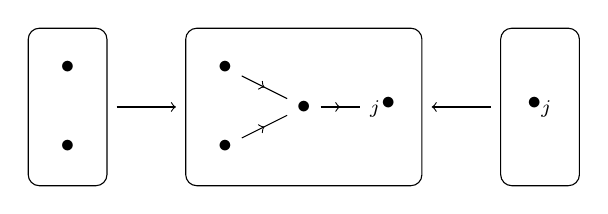
\begin{tikzpicture}
       %
      \begin{scope} % left graph
      \node (1) at (0,1) { \( \bullet \) };
      \node (2) at (0,0) { \( \bullet \) };
      \draw [rounded corners] (-0.5,-0.5) rectangle (0.5,1.5);
      \end{scope}
      %
      \begin{scope}[shift={(2,0)}] % center graph
      \node (1) at (0,1) {\( \bullet \)};
      \node (2) at (0,0) {\( \bullet \)};
      \node (3) at (1,0.5) {\( \bullet  \)};
      \node (4) at (2,0.5) {\( {}_{j} \bullet  \)};
      \draw [->-] (1) to (3);
      \draw [->-] (2) to (3);
      \draw [->-] (3) to (4);
      \draw [rounded corners] (-0.5,-0.5) rectangle (2.5,1.5);
      \end{scope}
      %
      \begin{scope}[shift={(6,0)}] % right graph
      \node (1) at (0,0.5) {\( \bullet_{j} \)};
      \draw [rounded corners] (-0.5,-0.5) rectangle (0.5,1.5);
      \end{scope}
      %
      \begin{scope} % graph morphisms
      \node (1) at (0.5,0.5) {};
      \node (2) at (1.5,0.5) {};
      \node (3) at (4.5,0.5) {};
      \node (4) at (5.5,0.5) {};
      \draw [->] (1) to (2);
      \draw [->] (4) to (3);
      \end{scope}
      %
    \end{tikzpicture}
  \]
  % 
  with
   %
  \[
    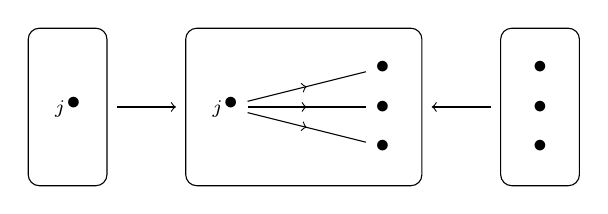
\begin{tikzpicture}
       %
      \begin{scope} % left graph
      \node (1) at (0,0.5) { \( {}_{j} \bullet \) };
      \draw [rounded corners] (-0.5,-0.5) rectangle (0.5,1.5);
      \end{scope}
      %
      \begin{scope}[shift={(2,0)}] % center graph
      \node (1) at (0,0.5) {\( {}_{j} \bullet \)};
      \node (2) at (2,0) {\( \bullet \)};
      \node (3) at (2,0.5) {\( \bullet  \)};
      \node (4) at (2,1) {\( \bullet  \)};
      \draw [->-] (1) to (2);
      \draw [->-] (1) to (3);
      \draw [->-] (1) to (4);
      \draw [rounded corners] (-0.5,-0.5) rectangle (2.5,1.5);
      \end{scope}
      %
      \begin{scope}[shift={(6,0)}] % right graph
      \node (2) at (0,0) {\( \bullet \)};
      \node (3) at (0,0.5) {\( \bullet  \)};
      \node (4) at (0,1) {\( \bullet  \)};
      \draw [rounded corners] (-0.5,-0.5) rectangle (0.5,1.5);
      \end{scope}
      %
      \begin{scope} % graph morphisms
      \node (1) at (0.5,0.5) {};
      \node (2) at (1.5,0.5) {};
      \node (3) at (4.5,0.5) {};
      \node (4) at (5.5,0.5) {};
      \draw [->] (1) to (2);
      \draw [->] (4) to (3);
      \end{scope}
      %
    \end{tikzpicture}
  \]
  %
  to get the open graph
  %
  \[
    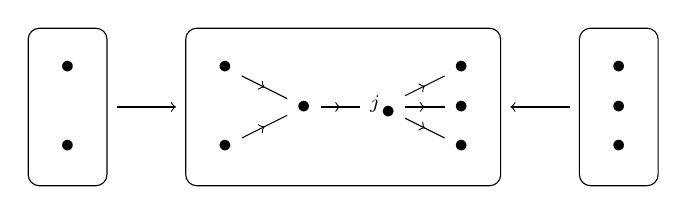
\begin{tikzpicture}
       %
      \begin{scope} % left graph
      \node (1) at (0,1) { \( \bullet \) };
      \node (2) at (0,0) { \( \bullet \) };
      \draw [rounded corners] (-0.5,-0.5) rectangle (0.5,1.5);
      \end{scope}
      %
      \begin{scope}[shift={(2,0)}] % center graph
      \node (1) at (0,1) {\( \bullet \)};
      \node (2) at (0,0) {\( \bullet \)};
      \node (3) at (1,0.5) {\( \bullet  \)};
      \node (4) at (2,0.5) {\( {}^{j} \bullet  \)};
      \node (5) at (3,0) {\( \bullet \)};
      \node (6) at (3,0.5) {\( \bullet  \)};
      \node (7) at (3,1) {\( \bullet  \)};
      \draw [->-] (1) to (3);
      \draw [->-] (2) to (3);
      \draw [->-] (3) to (4);
      \draw [->-] (4) to (5);
      \draw [->-] (4) to (6);
      \draw [->-] (4) to (7);
      \draw [rounded corners] (-0.5,-0.5) rectangle (3.5,1.5);
      \end{scope}
      %
      \begin{scope}[shift={(7,0)}] % right graph
      \node (2) at (0,0) {\( \bullet \)};
      \node (3) at (0,0.5) {\( \bullet  \)};
      \node (4) at (0,1) {\( \bullet  \)};
      \draw [rounded corners] (-0.5,-0.5) rectangle (0.5,1.5);
      \end{scope}
      %
      \begin{scope} % graph morphisms
      \node (1) at (0.5,0.5) {};
      \node (2) at (1.5,0.5) {};
      \node (3) at (5.5,0.5) {};
      \node (4) at (6.5,0.5) {};
      \draw [->] (1) to (2);
      \draw [->] (4) to (3);
      \end{scope}
      %
    \end{tikzpicture}
  \]
  %
  which is obtained by glueing the two open graphs together
  along the node $ j $.
  
\end{example}

% ~~~~~~~~~~~~~~~~~~~~~~~~
% ~~~~~~~~~~~~~~~~~~~~~~~~

\subsection{Structured cospans as objects}
\label{sec:StrCspAsObject}

A morphism of open systems ought to respect the system plus
its inputs and outputs.

\begin{definition} \label{df:morph-of-strcsp}

  A morphism between $ L $-structured cospans
  \( \csp{La}{x}{Lb} \) and \( \csp{Lc}{y}{Ld} \) is a
  triple of arrows $ ( f,g,h ) $ that fit into the commuting
  diagram
  \[
    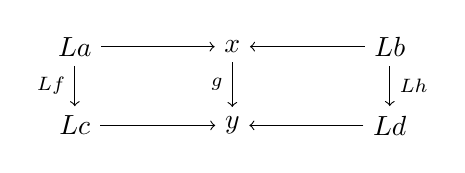
\begin{tikzpicture}
      \node (1) at (-2,1) {\( La \)};
      \node (2) at (0,1) {\( x \)};
      \node (3) at (2,1) {\( Lb \)};
      \node (4) at (-2,0) {\( Lc \)};
      \node (5) at (0,0) {\( y \)};
      \node (6) at (2,0) {\( Ld \)};
      \draw [->] (1) to node [above] {\scriptsize{\(  \)}} (2);
      \draw [->] (3) to node [above] {\scriptsize{\(  \)}} (2);
      \draw [->] (4) to node [below] {\scriptsize{\(  \)}} (5);
      \draw [->] (6) to node [below] {\scriptsize{\(  \)}} (5);
      \draw [->] (1) to node [left] {\scriptsize{\( Lf \)}} (4);
      \draw [->] (2) to node [left] {\scriptsize{\( g \)}} (5);
      \draw [->] (3) to node [right] {\scriptsize{\( Lh \)}} (6);
    \end{tikzpicture}
  \]
\end{definition}

It is easy to check that $ L $-structured cospans and their
morphisms form a category, which we denote by
$ _{L}\StrCsp $.

We now come to the first of our main results: that
$ _{L}\StrCsp $ is a topos. This result is critical for our
theory because it allows the introduction of rewriting onto
structured cospans.

\begin{theorem}
\label{thm:strcsp-istopos}
For any geometric morphism $ L \dashv R \from \A \to \X $,
the category $ _{L}\StrCsp $ is a topos.
\end{theorem}

\begin{proof}
  Note that $ _{L}\StrCsp $ is equivalent to the category
  whose objects are cospans of form
  %
  \(
    \csp{a}{Rx}{b}
  \)
  % 
  and morphisms are triples $ ( f,g,h ) $ fitting into the
  commuting diagram
  %
  \[
    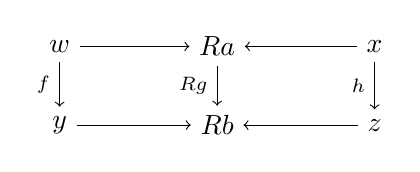
\begin{tikzpicture}
      \node (1) at (-2,1) {\( w \)};
      \node (2) at (0,1) {\( Ra \)};
      \node (3) at (2,1) {\( x \)};
      \node (4) at (-2,0) {\( y \)};
      \node (5) at (0,0) {\( Rb \)};
      \node (6) at (2,0) {\( z \)};
      \draw [->] (1) to  node [] {\scriptsize{\(  \)}} (2);
      \draw [->] (3) to node [] {\scriptsize{\(  \)}} (2);
      \draw [->] (4) to node [] {\scriptsize{\(  \)}} (5);
      \draw [->] (6) to node [] {\scriptsize{\(  \)}} (5);
      \draw [->] (1) to node [left] {\scriptsize{\( f \)}} (4);
      \draw [->] (2) to node [left] {\scriptsize{\( Rg \)}} (5);
      \draw [->] (3) to node [left] {\scriptsize{\( h \)}} (6); 
    \end{tikzpicture}
  \]
  % 
  This, in turn, is equivalent to the comma category
  $ ( \A \times \A \downarrow \Delta R ) $, where
  $ \Delta \from \A \to \A \times \A $ is the diagonal
  functor. But the diagonal functor is right adjoint to the
  coproduct functor. Therefore, $ \Delta R $ is also a right
  adjoint so $ ( \A \times \A \downarrow \Delta R ) $ is an
  instance of Artin gluing \cite{Wraith_ArtinGlue}, hence a
  topos.
\end{proof}

We now show that constructing $ _{L}\StrCsp $ is functorial.

\begin{theorem} \label{thm:strcsp-isfunctorial}
  There is a functor
  %
  \[
    _{(-)}\StrCsp_{(-)} \from
    [ \bullet \to \bullet , \Topos ]
    \to
    \Topos
  \]
  % 
  defined by  
  \[
    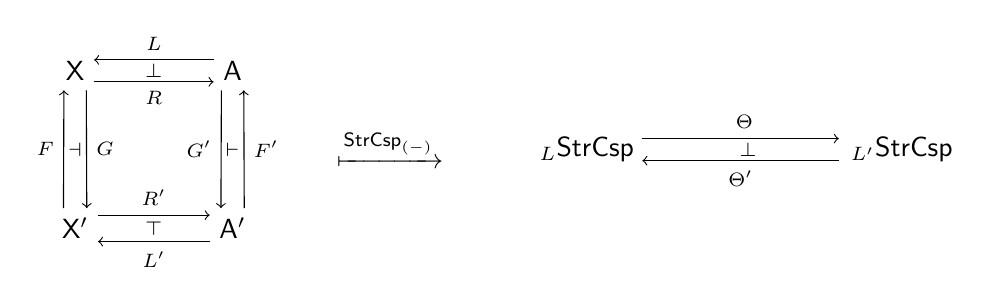
\begin{tikzpicture}
      \begin{scope}
        \node (1) at (-1,1) {\( \X \)}; \node (2) at (-1,-1)
        {\( \X' \)}; \node (3) at (1,1) {\( \A \)}; \node
        (4) at (1,-1) {\( \A' \)}; \draw [->] (1.-60) to
        node [right] {\scriptsize{\( G \)}} (2.60); \draw
        [<-] (1.-120) to node [left] {\scriptsize{\( F \)}}
        (2.120); \draw [<-] (1.30) to node [above]
        {\scriptsize{\( L \)}} (3.150); \draw [->] (1.-30)
        to node [below] {\scriptsize{\( R \)}} (3.-150);
        \draw [->] (2.30) to node [above]
        {\scriptsize{\( R' \)}} (4.150); \draw [<-] (2.-30)
        to node [below] {\scriptsize{\( L' \)}} (4.-150);
        \draw [<-] (3.-60) to node [right]
        {\scriptsize{\( F' \)}} (4.60); \draw [->] (3.-120)
        to node [left] {\scriptsize{\( G' \)}} (4.120);
        \node (5) at (0,-1) {\scriptsize{\( \top \)}}; \node
        (6) at (0,1) {\scriptsize{\( \perp \)}}; \node (7)
        at (-1,0) {\scriptsize{\( \dashv \)}}; \node (8) at
        (1,0) {\scriptsize{\( \vdash \)}};
      \end{scope}
     % 
      \begin{scope}[shift={(3,0)}]
      \node (1) at (0,0) { $\xmapsto{ \StrCsp_{(-)} }$ };
      \end{scope}
      %
      \begin{scope}[shift={(5.5,0)}]
      \node (1) [inner sep=0.1cm] at (0,0) {\( _{L}\StrCsp \)};
      \node (2) [inner sep=0.15cm] at (4,0) {\( _{L'}\StrCsp \)};
      \node (3) at (2,0) {\scriptsize{ \( \perp \) }};
      \draw [->]
        ([yshift= 4pt]1.east) to
        node [above] {\scriptsize{ \( \Theta \) }}
        ([yshift= 4pt]2.west);
      \draw [->]
        ([yshift= -4pt]2.west) to
        node [below] {\scriptsize{ \( \Theta' \) } }
        ([yshift= -4pt]1.east);  
      \end{scope}
    \end{tikzpicture}
  \]
  % 
  which is in turn given by
  %
  \[
    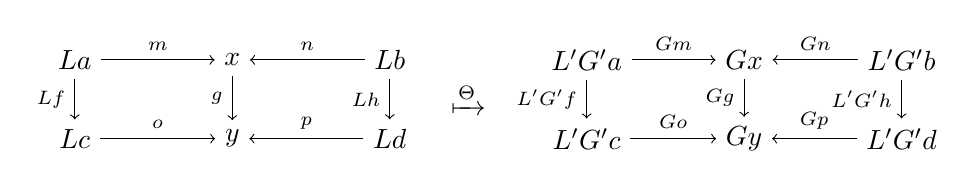
\begin{tikzpicture}
      \begin{scope}
      \node (1) at (-2,1) {\( La \)};
      \node (2) at (0,1) {\( x \)};
      \node (3) at (2,1) {\( Lb \)};
      \node (4) at (-2,0) {\( Lc \)};
      \node (5) at (0,0) {\( y \)};
      \node (6) at (2,0) {\( Ld \)};
      \draw [->] (1) to node [above] {\scriptsize{\( m \)}} (2);
      \draw [->] (3) to node [above] {\scriptsize{\( n \)}} (2);
      \draw [->] (4) to node [above] {\scriptsize{\( o \)}} (5);
      \draw [->] (6) to node [above] {\scriptsize{\( p \)}} (5);
      \draw [->] (1) to node [left] {\scriptsize{\( Lf \)}} (4);
      \draw [->] (2) to node [left] {\scriptsize{\( g \)}} (5);
      \draw [->] (3) to node [left] {\scriptsize{\( Lh \)}} (6);
      \end{scope}
      %
      \begin{scope}[shift={(3,0)}]
      \node (1) at (0,0.5) { $ \xmapsto{ \Theta } $ };
      \end{scope}
      %
      \begin{scope}[shift={(6.5,0)}]
      \node (1) at (-2,1) {\( L'G'a \)};
      \node (2) at (0,1) {\( Gx \)};
      \node (3) at (2,1) {\( L'G'b \)};
      \node (4) at (-2,0) {\( L'G'c \)};
      \node (5) at (0,0) {\( Gy \)};
      \node (6) at (2,0) {\( L'G'd \)};
      \draw [->] (1) to node [above] {\scriptsize{\( Gm \)}} (2);
      \draw [->] (3) to node [above] {\scriptsize{\( Gn \)}} (2);
      \draw [->] (4) to node [above] {\scriptsize{\( Go \)}} (5);
      \draw [->] (6) to node [above] {\scriptsize{\( Gp \)}} (5);
      \draw [->] (1) to node [left] {\scriptsize{\( L'G'f \)}} (4);
      \draw [->] (2) to node [left] {\scriptsize{\( Gg \)}} (5);
      \draw [->] (3) to node [left] {\scriptsize{\( L'G'h \)}} (6);  
      \end{scope}
    \end{tikzpicture}
  \]
  %
  and
  %
  \[
    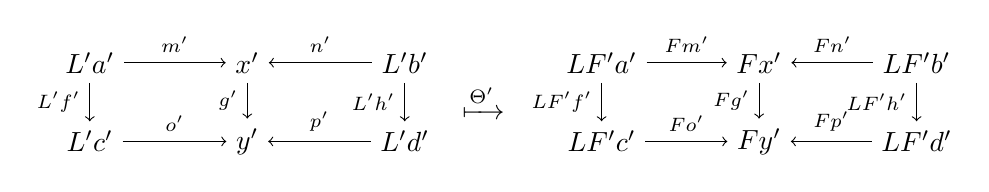
\begin{tikzpicture}
      \begin{scope}
      \node (1) at (-2,1) {\( L'a' \)};
      \node (2) at (0,1) {\( x' \)};
      \node (3) at (2,1) {\( L'b' \)};
      \node (4) at (-2,0) {\( L'c' \)};
      \node (5) at (0,0) {\( y' \)};
      \node (6) at (2,0) {\( L'd' \)};
      \draw [->] (1) to node [above] {\scriptsize{\( m' \)}} (2);
      \draw [->] (3) to node [above] {\scriptsize{\( n' \)}} (2);
      \draw [->] (4) to node [above] {\scriptsize{\( o' \)}} (5);
      \draw [->] (6) to node [above] {\scriptsize{\( p' \)}} (5);
      \draw [->] (1) to node [left] {\scriptsize{\( L'f' \)}} (4);
      \draw [->] (2) to node [left] {\scriptsize{\( g' \)}} (5);
      \draw [->] (3) to node [left] {\scriptsize{\( L'h' \)}} (6);
      \end{scope}
      %
      \begin{scope}[shift={(3,0)}]
      \node (1) at (0,0.5) { $ \xmapsto{ \Theta' } $ };
      \end{scope}
      %
      \begin{scope}[shift={(6.5,0)}]
      \node (1) at (-2,1) {\( LF'a' \)};
      \node (2) at (0,1) {\( Fx' \)};
      \node (3) at (2,1) {\( LF'b' \)};
      \node (4) at (-2,0) {\( LF'c' \)};
      \node (5) at (0,0) {\( Fy' \)};
      \node (6) at (2,0) {\( LF'd' \)};
      \draw [->] (1) to node [above] {\scriptsize{\( Fm' \)}} (2);
      \draw [->] (3) to node [above] {\scriptsize{\( Fn' \)}} (2);
      \draw [->] (4) to node [above] {\scriptsize{\( Fo' \)}} (5);
      \draw [->] (6) to node [above] {\scriptsize{\( Fp' \)}} (5);
      \draw [->] (1) to node [left] {\scriptsize{\( LF'f' \)}} (4);
      \draw [->] (2) to node [left] {\scriptsize{\( Fg' \)}} (5);
      \draw [->] (3) to node [left] {\scriptsize{\( LF'h' \)}} (6);  
      \end{scope}
    \end{tikzpicture}
  \]  
\end{theorem}

\begin{proof}
  In light of Theorem \ref{thm:strcsp-istopos}, it suffices
  to show that $ \Theta \dashv \Theta' $ gives a geometric
  morphism.

  Denote the structured cospans
  %
  \[
    [ m,n ] \colon \csp{La}{x}{Lb}
  \]
  % 
  in $ \StrCsp_{ L } $ by $ \ell $ and  
  %
  \[
    [m',n'] \colon \csp{L'a'}{x'}{L'b'}
  \]
  % 
  in $ \StrCsp_{ L' } $ by $ \ell' $. Denote the unit and
  counit for $F \dashv G$ by $ \eta $, $ \varepsilon $ and
  for $ F' \dashv G' $ by $ \eta' $, $ \varepsilon' $.  The
  assignments
  %
  \begin{align*}
    \left(
      ( f,g,h ) \from \ell \to \Theta' \ell'
      \right)
    & \mapsto
    \left(
      ( \varepsilon' \circ F'f , \varepsilon \circ Fg , \varepsilon'
      \circ F'h )
      \from \Theta \ell \to \ell'
      \right) \\
      %
      \left(
      ( f',g',h' ) \from \Theta \ell \to \ell'
      \right)
    & \mapsto
      \left(
      ( G'f' \circ \eta', Gg' \circ \eta , G'h' \circ \eta' )
      \from \ell \to \Theta' \ell'
      \right) 
  \end{align*}
  %
  give a bijection
  $ \hom ( \Theta \ell , \ell' ) \simeq \hom ( \ell ,
  \Theta' \ell' ) $. Moreover, it is natural in $ \ell $ and
  $ \ell' $. This rests on the natural maps $ \eta $,
  $ \varepsilon $, $ \eta' $, and $ \varepsilon' $. The left
  adjoint $ \Theta' $ preserves finite limits because they
  are taken pointwise and $ L $, $ F $, and $ F' $ all
  preserve finite limits.
\end{proof}

The morphisms $ _{L}\StrCsp \to _{L'}\StrCsp $ that we are
interested in act on the systems and their interfaces.

\begin{definition} \label{def:str-csp-functor}
  A \defn{structured cospan functor} is a pair of finitely
  continuous and cocontinuous functors
  $ F \from \X \to \X' $ and $ G \from \A \to \A' $ such
  that $ FL=L'F $ and $ GR = R'F $.
\end{definition}

Structured cospan categories and their morphisms form a
category which we leave unnamed.

% ~~~~~~~~~~~~~~~~~~~~~~~~
% ~~~~~~~~~~~~~~~~~~~~~~~~

\subsection{A double category of structured cospans}
\label{sec:DblCatOfStrCsp}

We use (pseudo) double categories to combine into a single
instrument the competing perspectives of structured cospans
as objects and as morphisms. For a precise definition of a
double category, we point to Shulman \cite{ShulDblCat},
though we list the key components for the sake of
completeness. A \emph{(pseudo) double category} $ \CCC $ is
a category weakly internal to $ \Cat $, which roughly
translates to a category of objects $ \CCC_0 $ together with
a category of arrows $ \CCC_1 $ that assemble together
as follows.
% 
\begin{itemize}
\item The $ \CCC_0 $-objects are called the objects of
  $ \CCC $.
\item The $ \CCC_0 $-arrows are called the vertical arrows in
  $ \CCC $.
\item The $ \CCC_1 $-objects are called the the horizontal
  arrows in $ \CCC $.
\item The $ \CCC_1 $-arrows are called the squares of $ \CCC $.
are the arrows of $ \CCC_1 $. 
\end{itemize}
%
See Figure \ref{fig:square} for a depiction of this data.

\begin{figure}[h]
  \centering
  \[
  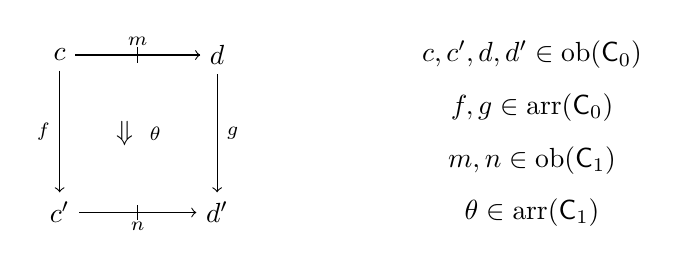
\begin{tikzpicture}
    \node (1) at (0,2) {\( c \)};
    \node (2) at (2,2) {\( d \)};
    \node (3) at (0,0) {\( c' \)};
    \node (4) at (2,0) {\( d' \)};
    \draw [-|->] (1) to node [above] {\scriptsize{\( m \)}} (2);
    \draw [->] (1) to node [left] {\scriptsize{\( f \)}} (3);
    \draw [->] (2) to node [right] {\scriptsize{\( g \)}} (4);
    \draw [-|->] (3) to node [below] {\scriptsize{\( n \)}} (4);
    \node (5) at (6,2) {\( c,c',d,d' \in \operatorname{ob} ( \C_0 ) \)};
    \node (6) at (6,1.33) {\( f,g \in \operatorname{arr} ( \C_0 ) \)};
    \node (7) at (6,.66) {\( m,n \in \operatorname{ob} ( \C_1 ) \)};
    \node (8) at (1,1) {\( \Downarrow \) \scriptsize{ \( \theta \)}};
    \node (9) at (6,0) {\( \theta \in \operatorname{arr} ( \C_1 ) \)};
  \end{tikzpicture}
\]
  \caption{A square in a double category}
  \label{fig:square}
\end{figure}

In addition, there are structure maps ensuring the correct
interplay between the elements of this data.  The vertical
arrows compose as they do in $ \CCC_0 $ and there is a
structure map for composing horizontal arrows. The squares
compose horizontally and vertically and, moreover, an
interchange law ensures the proper interplay of these
compositions.

Observe that the horizontal arrows play two roles: as
objects in their category of origin and as arrows in the
double category. This reinforces our choice to organize
structured cospans in a double category.

\begin{definition}
  There is a double category
  $ _{L}\SSStrCsp \coloneqq ( \A , _{L}\StrCsp ) $ :
  \begin{itemize}
  \item the objects are the $ \A $-objects
  \item the vertical arrows $ a \to b $ the $ \A $-arrows, 
  \item the horizontal arrows $ a \horarrow b $ are the cospans
    $ \csp{La}{x}{Lb} $, and
  \item the squares are the commuting diagrams
    %
    \[
    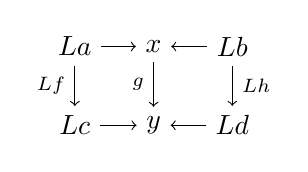
\begin{tikzpicture}
    \node (1) at (0,1) {\( La \)};
    \node (2) at (1,1) {\( x \)};
    \node (3) at (2,1) {\( Lb \)};
    \node (4) at (0,0) {\( Lc \)};
    \node (5) at (1,0) {\( y \)};
    \node (6) at (2,0) {\( Ld \)};
    \draw [->] (1) to node [] {\scriptsize{\(   \)}} (2);
    \draw [->] (3) to node [] {\scriptsize{\(  \)}} (2);
    \draw [->] (4) to node [] {\scriptsize{\(  \)}} (5);
    \draw [->] (6) to node [] {\scriptsize{\(  \)}} (5);
    \draw [->] (1) to node [left] {\scriptsize{\( Lf \)}} (4);
    \draw [->] (2) to node [left] {\scriptsize{\( g \)}} (5);
    \draw [->] (3) to node [right] {\scriptsize{\( Lh \)}} (6);
    \end{tikzpicture}
  \]
  \end{itemize}
  %  
\end{definition}

Baez and Courser proved that this truly is a double category
\cite[Cor.~3.9]{StrCsp}. Moreover, when $ \cat{ A } $ and
$ \cat{ X } $ are cocartesian, their coproducts can be used
to define a symmetric monoidal structure on
$ _{L}\SSStrCsp $. The meaning of this structure is that the
disjoint union of two systems can be considered a single
system. Because we have no need for this structure in this
paper, we say no more about it.


% ~~~~~~~~~~~~~~~~~~~~~~~~~~~~~~~~~~~~~~~~
% ~~~~~~~~~~~ rewriting ~~~~~~~~~~~~~~~~~~
% ~~~~~~~~~~~~~~~~~~~~~~~~~~~~~~~~~~~~~~~~

\section{Rewriting}
\label{sec:rewriting}

We begin this final section by recalling the basics of
double pushout rewriting within the context of topoi. We
also present the second of our main results: the
generalization of a result about the expressiveness of
certain graph grammars. We apply this rewriting theory to
structured cospans. In doing so, we show the rewrite
relation is functorial. This section also contains our main
result which is a generalization of work by Gadducci and
Heckle \cite{Gadd_IndGraphTrans}.  Yet, this result is not a
mere generalization but provides a justification the study
of systems using structured cospans.

Ehrig, et.\ al.\ \cite{Ehrig_GraphGram} invented double pushout rewriting on graphs. It has since undergone
extensive study and generalization. Currently, the most
general setting to contain a rich theory of rewriting is
adhesive categories, introduced by Lack and Soboci\'{n}ski
\cite{LackSobo_Adhesive}. Topoi are examples of adhesive
categories \cite{LackSobo_ToposIsAdh} so it follows that we
can bring a theory of rewriting to structured cospans.


\subsection{Rewriting in topoi}
\label{sec:Adhesive-Rewriting}

Fix a topos $ \C $.  Rewriting starts with the notion of a
\defn{rewrite rule}, or simply \defn{rule}.  This is a span
%
\[
  \ell \monicgets k \monicto r
\]
% 
in $ \C $ with monic legs. We continue to denote spans by
$ \spn{\ell}{k}{r} $ with the the caveat that, whenever we say that a
span is a rule, we understand that both legs are
monic. The conceit of a rule is that $ r $ replaces $ \ell $ while the common subobject $ k $ remains fixed. We can
apply this rule to objects $ m \from \ell \monicto g $
having $ \ell $ as a subobject if there exists a
\defn{pushout complement}, that is an object $ d $ fitting
into a pushout diagram
% 
\[
  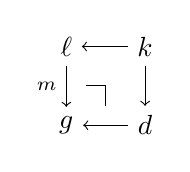
\begin{tikzpicture}
    \node (l) at (0,1) {$ \ell $};
    \node (k) at (1,1) {$ k $};
    \node (g) at (0,0) {$ g $};
    \node (d) at (1,0) {$ d $};
    \draw [->] (k) to node [] {\scriptsize{$  $}} (l);
    \draw [->] (d) to node [] {\scriptsize{$  $}} (g);
    \draw [->] (l) to node [left] {\scriptsize{$ m $}} (g);
    \draw [->] (k) to node [] {\scriptsize{$  $}} (d);
    % corners
    \begin{scope}[shift={(0,0)}]
      % \draw [-] (0,0) to (0,0.25);
      \draw [-] (0.25,0.5) to node [] {} (0.5,0.5);
      \draw [-] (0.5,0.5) to node [] {} (0.5,0.25);
    \end{scope}
  \end{tikzpicture}
\]
% 
A pushout complement need not exist, but when it does and
the map $ k \to \ell $ is monic, then it is unique up to
isomorphism \cite[Lem.~15]{LackSobo_Adhesive}.

Given a rule $ \spn{l}{k}{r} $ together with a suitable
$ \ell \monicto g $, we obtain a \defn{derived rule}
$ \spn{g}{d}{h} $ on the bottom row of the \emph{double
  pushout diagram}
%
\[
  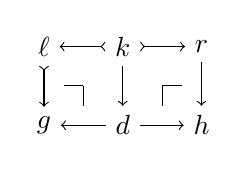
\begin{tikzpicture}
    \node (1) at (0,1) {$ \ell $};
    \node (2) at (1,1) {$ k $};
    \node (3) at (2,1) {$ r $};
    \node (4) at (0,0) {$ g $};
    \node (5) at (1,0) {$ d $};
    \node (6) at (2,0) {$ h $};
    \draw [>->] (2) to node [] {\scriptsize{$  $}} (1);
    \draw [>->] (2) to node [] {\scriptsize{$  $}} (3);
    \draw [->] (5) to node [] {\scriptsize{$  $}} (4);
    \draw [->] (5) to node [] {\scriptsize{$  $}} (6);
    \draw [>->] (1) to node [] {\scriptsize{$  $}} (4);
    \draw [->] (2) to node [] {\scriptsize{$  $}} (5);
    \draw [->] (3) to node [] {\scriptsize{$  $}} (6);
     \begin{scope}[shift={(0,0)}]
      % \draw [-] (0,0) to (0,0.25);
      \draw [-] (0.25,0.5) to node [] {} (0.5,0.5);
      \draw [-] (0.5,0.5) to node [] {} (0.5,0.25);
    \end{scope}
    %
     \begin{scope}[shift={(1.5,0)}]
      \draw [-] (0,0.25) to (0,0.5);
      \draw [-] (0,0.5) to node [] {} (0.25,0.5);
      % \draw [-] (0.5,0.5) to node [] {} (0.5,0.25);
    \end{scope}
  \end{tikzpicture}
\]
%
The span $ \spn{g}{d}{h} $ is a rule because pushouts
preserve monics in topoi
\cite[Lem.~12]{LackSobo_Adhesive}. The intuition of this
diagram is that $ \ell \monicto g $ gives an instance of
$ \ell $ in $ g $ which $ r $ replaces, resulting in a new object $ h $.

A topos $ \C $ together with a finite set $ P $ of rules
$ \{ \spn{\ell_j}{k_j}{r_j} \} $ in $ \cat{ C } $ is 
a \defn{grammar}. An arrow of grammars
$ ( \C , P ) \to ( \D , Q ) $ is a monic preserving functor
$ F \from \C \to \D $ such that for each rule
$ \langle f,g \rangle \from \spn{\ell}{k}{r} $ in $ P $, the
rule $ \langle Ff,Fg \rangle \from \spn{F\ell}{Fk}{Fr} $ is
isomorphic to a rule in $ Q $. Together these form a
category $ \Gram $.

Every grammar $ ( \C , P ) $ gives rise to a relation
$ \deriv{}{} $ on the objects of $ \C $ defined by
$ \dderiv{g}{h} $ whenever there exists a rule
$ \spn{g}{d}{h} $ derived from a production in $ P
$. But this relation is too small to capture the full
behavior induced by a grammar.  For one, it is not true in
general that $ \dderiv{x}{x} $ holds. Also, it doesn't
capture multi-step rewrites. That is, there may be
derived rules witnessing $ \dderiv{g}{g'} $ and
$ \dderiv{g'}{g''} $ but not a derived rule witnessing
$ \dderiv{g}{g''} $. Yet, we want to be able to relate a
pair of objects if one can be rewritten into another with a
finite sequence of derived rules. So, the relation we
actually want is the reflexive and transitive closure of
$ \rightsquigarrow $, which we denote by
$ \rightsquigarrow^\ast $.  This, we call the \defn{rewrite
  relation}.  Every grammar determines a unique rewrite
relation in a functorial way.  Though, restrict our attention to showing this
in the context of structured cospan categories.


\subsection{Expressiveness of underlying discrete grammars}
\label{sec:gen-result-graph-rewriting}

In this section, we generalize a result
\cite[Prop.~3.3]{Ehrig_GraphGram} from the theory of
rewriting graphs into the theory of rewriting in topoi.

The statement of this result, in our current context, begins
with the underlying discrete graph comonad
$ \flat \from \RGraph \to \RGraph $. The monic counit
$ \flat g \monicto g $ includes the underlying discrete
graph $ \flat g $ into $ g $.  Given a grammar
$ ( \RGraph , P ) $, define a new grammar
$ ( \RGraph , P_\flat ) $ where $ P_\flat $ consists of
rules $ k_\flat \hookrightarrow k \to \ell \times r $ for
each rule $ \spn{\ell}{k}{r} $ in $ P $. Then a graph $ g $
is related to a graph $ h $ with respect to the rewrite
relation induced by $ ( \RGraph , P ) $ if and only if $ g $
is related to $ h $ with respect to the rewriting relation
induced by $ ( \RGraph , P_\flat ) $.

To generalize this result, we first settle a few things.
Fix a geometric morphism $ L \dashv R \from \X \to \A
$. Denote by $ ( \X , P_\flat ) $ the \defn{discrete
  grammar} underlying $ ( \X , P ) $. This consists of all
rules obtained by pulling back $ k \to \ell \times r $ by
the counit $ LRk \to k $ for each rule in $ P $.

Recall that a poset is \textbf{well-founded} if every
non-empty subset has a minimal element.  Whenever the axiom
of choice is present, well-foundedness is equivalent to a
lack of infinite descending chains.

\begin{example}
  As the axiom of choice holds in any presheaf category, the
  Heyting algebra $ \Sub ( x ) $ for any finite-set valued
  presheaf $ x $ is well-founded. In the case of
  $ \RGraph $, the subobject algebra of any finite graph is
  well-founded.
\end{example}

\begin{theorem}
\label{thm:production-same-rewrite-relation-as-discrete}
Fix a geometric morphism $ L \dashv R \from \X \to \A $ with
monic counit. Let $ ( \X , P ) $ be a grammar such that for
every $ \X $-object $ x $ in the apex of a production of
$ P $, the Heyting algebra $ \Sub (x) $ is well-founded.
The rewriting relation for a grammar $ ( \X , P ) $ is equal
to rewriting relation for the grammar $ ( \X , P_{\flat} ) $
\end{theorem}

\begin{proof}
  For any derivation
  %
  \[
  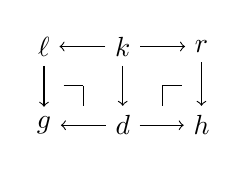
\begin{tikzpicture}
    \node (1t) at (0,1) {$ \ell $};
    \node (2t) at (1,1) {$ k $};
    \node (3t) at (2,1) {$ r $};
    \node (1b) at (0,0) {$ g $};
    \node (2b) at (1,0) {$ d $};
    \node (3b) at (2,0) {$ h $};
    \draw [->] (2t) to node [] {\scriptsize{$  $}} (1t);
    \draw [->] (2t) to node [] {\scriptsize{$  $}} (3t);
    \draw [->] (2b) to node [] {\scriptsize{$  $}} (1b);
    \draw [->] (2b) to node [] {\scriptsize{$  $}} (3b);
    \draw [->] (1t) to node [] {\scriptsize{$  $}} (1b);
    \draw [->] (2t) to node [] {\scriptsize{$  $}} (2b);
    \draw [->] (3t) to node [] {\scriptsize{$  $}} (3b);
     \begin{scope}[shift={(0,0)}]
      % \draw [-] (0,0) to (0,0.25);
      \draw [-] (0.25,0.5) to node [] {} (0.5,0.5);
      \draw [-] (0.5,0.5) to node [] {} (0.5,0.25);
    \end{scope}
    \begin{scope}[shift={(1.5,0)}]
      \draw [-] (0,0.25) to (0,0.5);
      \draw [-] (0,0.5) to node [] {} (0.25,0.5);
      % \draw [-] (0.5,0.5) to node [] {} (0.5,0.25);
    \end{scope}
  \end{tikzpicture}
  \]
  % 
  arising from $ P $, there is a derivation
  %
  \[
  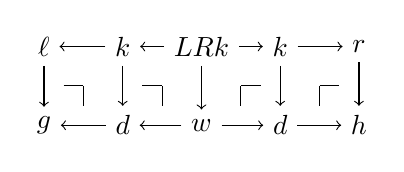
\begin{tikzpicture}
    \node (01) at (0,1) {$ \ell $};
    \node (11) at (1,1) {$ k $};
    \node (21) at (2,1) {$ LRk $};
    \node (31) at (3,1) {$ k $};
    \node (41) at (4,1) {$ r $};
    \node (00) at (0,0) {$ g $};
    \node (10) at (1,0) {$ d $};
    \node (20) at (2,0) {$ w $};
    \node (30) at (3,0) {$ d $};
    \node (40) at (4,0) {$ h $};
    \draw [->] (11) to node [] {\scriptsize{$  $}} (01);
    \draw [->] (21) to node [] {\scriptsize{$  $}} (11);
    \draw [->] (21) to node [] {\scriptsize{$  $}} (31);
    \draw [->] (31) to node [] {\scriptsize{$  $}} (41);
    \draw [->] (10) to node [] {\scriptsize{$  $}} (00);
    \draw [->] (20) to node [] {\scriptsize{$  $}} (10);
    \draw [->] (20) to node [] {\scriptsize{$  $}} (30);
    \draw [->] (30) to node [] {\scriptsize{$  $}} (40);
    \draw [->] (01) to node [] {\scriptsize{$  $}} (00);
    \draw [->] (11) to node [] {\scriptsize{$  $}} (10);
    \draw [->] (21) to node [] {\scriptsize{$  $}} (20);
    \draw [->] (31) to node [] {\scriptsize{$  $}} (30);
    \draw [->] (41) to node [] {\scriptsize{$  $}} (40);
    \begin{scope}[shift={(0,0)}]
      % \draw [-] (0,0) to (0,0.25);
      \draw [-] (0.25,0.5) to node [] {} (0.5,0.5);
      \draw [-] (0.5,0.5) to node [] {} (0.5,0.25);
    \end{scope}
    \begin{scope}[shift={(1,0)}]
      % \draw [-] (0,0) to (0,0.25);
      \draw [-] (0.25,0.5) to node [] {} (0.5,0.5);
      \draw [-] (0.5,0.5) to node [] {} (0.5,0.25);
    \end{scope}
    \begin{scope}[shift={(2.5,0)}]
      \draw [-] (0,0.25) to (0,0.5);
      \draw [-] (0,0.5) to node [] {} (0.25,0.5);
    \end{scope}
    \begin{scope}[shift={(3.5,0)}]
      \draw [-] (0,0.25) to (0,0.5);
      \draw [-] (0,0.5) to node [] {} (0.25,0.5);
    \end{scope}
  \end{tikzpicture}
  \]
  %
  where 
  %
  \[
    w \coloneqq
    \bigwedge \{ z \colon z \wedge k = x \} \vee LRk.
  \]
  Note that $ w \vee k = x $ and $ w \wedge k = LRy $ which
  gives that the two inner squares of the lower diagram are
  pushouts.
\end{proof}

% % ~~~~~~~~~~~~~~~~~~~~~~~~
% % ~~~~~~~~~~~~~~~~~~~~~~~~

\subsection{Rewriting structured cospans}
\label{sec:Rewriting-StrCsp}

We now apply rewriting in topoi to rewriting structured
cospans which is possible because of Theorem
\ref{thm:strcsp-istopos}.

There is a subcategory $ \StrCspGram $ of $ \Gram $ whose
objects are $ ( _{L}\StrCsp , P ) $ where $ P $ consists of
rules of the form
 %
 \[
   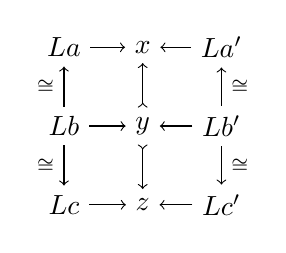
\begin{tikzpicture}
    \begin{scope}
        \node (1) at (0,2) {\( La \)};
        \node (2) at (1,2) {\( x \)};
        \node (3) at (2,2) {\( La' \)};
        \node (4) at (0,1) {\( Lb \)};
        \node (5) at (1,1) {\( y \)};
        \node (6) at (2,1) {\( Lb' \)};
        \node (7) at (0,0) {\( Lc \)};
        \node (8) at (1,0) {\( z \)};
        \node (9) at (2,0) {\( Lc' \)};
        \draw [->] (1) to node []
          {\scriptsize{\( \)}} (2);
        \draw [->] (3) to node []
          {\scriptsize{\( \)}} (2);
        \draw [->] (4) to node []
          {\scriptsize{\( \)}} (5);
        \draw [->] (6) to node []
          {\scriptsize{\( \)}} (5);
        \draw [->] (7) to node []
          {\scriptsize{\( \)}} (8);
        \draw [->] (9) to node []
          {\scriptsize{\( \)}} (8);
        \draw [->] (4) to node [left]
          {\scriptsize{\( \iso \)}} (1);
        \draw [->] (4) to node [left]
          {\scriptsize{\( \iso \)}} (7);
        \draw [>->] (5) to node []
          {\scriptsize{\( \)}} (2);
        \draw [>->] (5) to node []
          {\scriptsize{\( \)}} (8);
        \draw [->] (6) to node [right]
          {\scriptsize{\( \iso \)}} (3);
        \draw [->] (6) to node [right]
          {\scriptsize{\( \iso \)}} (9);
    \end{scope}
  \end{tikzpicture}
\]
%
and the morphisms are the structured cospan functors
(Definition \ref{def:str-csp-functor}) that are stable under
the grammars. The objects run through $ L $ and $ P $.

Recall we associate a relation $ \rightsquigarrow $ to each
grammar, then take its reflexive and transitive closure to
get the rewrite relation $ \rightsquigarrow^\ast $. We now
show that this is a functor via a composite of
two functors, $ D \from \StrCspGram \to \StrCspGram $ and
$ S \from \StrCspGram \to \DblCat $, which we now define.

\begin{lemma}
  There is an idempotent functor
  $ D \from \StrCspGram \to \StrCspGram $. On
  objects define $ D ( _{L}\StrCsp , P ) $ to be the
  grammar $ ( _{L}\StrCsp , P') $, where $ P' $ consists of
  all rules $ \spn{g}{h}{d} $ witnessing the relation
  $ \dderiv{g}{h} $ with respect to $ ( _{L}\StrCsp , P )
  $. On arrows, define
  $ DF \from D( _{L}\StrCsp , P ) \to D( _{L'}\StrCsp , Q )
  $ to be $ F $.  Moreover, the identity on
  $ \StrCspGram $ is a subfunctor of $ D $.
\end{lemma}

\begin{proof}
  That $ D ( _{L}\StrCsp , P ) $ actually gives a grammar
  follows from the fact that pushouts respect monics in a
  topos \cite[Lem.~12]{LackSobo_Adhesive}.
  
  To show that $ \D $ is idempotent, we show that for any
  grammar $ ( _{L}\StrCsp , P ) $, we have
  $ D ( _{L}\StrCsp , P ) = DD ( _{L}\StrCsp , P ) $.  Rules
  in $ DD ( _{L}\StrCsp , P ) $ are the bottom row of a
  double pushout diagram whose top row is a rule in
  $ D ( _{L}\StrCsp , P ) $, which in turn is the bottom row
  of a double pushout diagram whose top row is in
  $ ( _{L}\StrCsp , P ) $. Thus, a rule in
  $ DD ( _{L}\StrCsp , P ) $ is the bottom row of a double
  pushout diagram whose top row is in
  $ ( _{L}\StrCsp , P ) $. See Figure \ref{fig:idempotentD}.

  \begin{figure}[h]
    \centering
    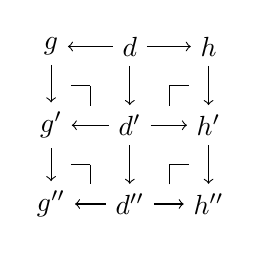
\begin{tikzpicture}
      \node (1) at (0,2) {$ g $};
      \node (2) at (1,2) {$ d $};
      \node (3) at (2,2) {$ h $};
      \node (4) at (0,1) {$ g' $};
      \node (5) at (1,1) {$ d' $};
      \node (6) at (2,1) {$ h' $};
      \node (7) at (0,0) {$ g'' $};
      \node (8) at (1,0) {$ d'' $};
      \node (9) at (2,0) {$ h'' $};
      \draw [->] (2) to node [] {\scriptsize{$  $}} (1);
      \draw [->] (2) to node [] {\scriptsize{$  $}} (3);
      \draw [->] (5) to node [] {\scriptsize{$  $}} (4);
      \draw [->] (5) to node [] {\scriptsize{$  $}} (6);
      \draw [->] (8) to node [] {\scriptsize{$  $}} (7);
      \draw [->] (8) to node [] {\scriptsize{$  $}} (9);
      \draw [->] (1) to node [] {\scriptsize{$  $}} (4);
      \draw [->] (2) to node [] {\scriptsize{$  $}} (5);
      \draw [->] (3) to node [] {\scriptsize{$  $}} (6);
      \draw [->] (4) to node [] {\scriptsize{$  $}} (7);
      \draw [->] (5) to node [] {\scriptsize{$  $}} (8);
      \draw [->] (6) to node [] {\scriptsize{$  $}} (9);
      \begin{scope}[shift={(0,0)}]
        % \draw [-] (0,0) to (0,0.25);
        \draw [-] (0.25,0.5) to node [] {} (0.5,0.5);
        \draw [-] (0.5,0.5) to node [] {} (0.5,0.25);
      \end{scope}
      \begin{scope}[shift={(0,1)}]
        % \draw [-] (0,0) to (0,0.25);
        \draw [-] (0.25,0.5) to node [] {} (0.5,0.5);
        \draw [-] (0.5,0.5) to node [] {} (0.5,0.25);
      \end{scope}
      \begin{scope}[shift={(1.5,0)}]
        \draw [-] (0,0.25) to (0,0.5);
        \draw [-] (0,0.5) to node [] {} (0.25,0.5);
        % \draw [-] (0.5,0.5) to node [] {} (0.5,0.25);
      \end{scope}
      \begin{scope}[shift={(1.5,1)}]
        \draw [-] (0,0.25) to (0,0.5);
        \draw [-] (0,0.5) to node [] {} (0.25,0.5);
        % \draw [-] (0.5,0.5) to node [] {} (0.5,0.25);
      \end{scope}
    \end{tikzpicture}
    \caption{Stacked double pushout diagrams}
    \label{fig:idempotentD}
  \end{figure}

    The identity is a subfunctor of $ D $ because
    $ \dderiv{\ell}{r} $ for any production
    $ \spn{\ell}{k}{r} $ in $ ( _{L}\StrCsp , P ) $ via a
    triple of identity arrows. Hence the identity functor on
    $ _{L}\StrCsp $ turns $ ( _{L}\StrCsp , P ) $ into a
    subobject of $ D ( _{L}\StrCsp , P ) $.
\end{proof}

This lemma sends each grammar to a new grammar consisting of
all derived rules.  That $ D $ is idempotent means that a
rule derived from a derived rule is derivable from the
original rule.  That identity is a subfunctor of $ D $ means
that the derived grammar contains all the rules of the
original grammar.

To define $ S $, we reference the double category
$ \MonSpCsp (\C) $ for a topos $ \C $ introduced in
\cite{CicCour_SpCspTopos}.  The objects are those in $ \C $,
the vertical arrows are spans with invertible legs in
$ \C $, the horizontal arrows are cospans in $ \C $, and the
squares are diagrams in $ \C $ with shape
%
\[
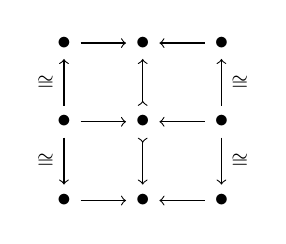
\begin{tikzpicture}
  \node (00) at (0,0) {$ \bullet $};
  \node (01) at (0,1) {$ \bullet $};
  \node (02) at (0,2) {$ \bullet $};
  \node (10) at (1,0) {$ \bullet $};
  \node (11) at (1,1) {$ \bullet $};
  \node (12) at (1,2) {$ \bullet $};
  \node (20) at (2,0) {$ \bullet $};
  \node (21) at (2,1) {$ \bullet $};
  \node (22) at (2,2) {$ \bullet $};
  \draw [->] (02) to node [] {\scriptsize{$  $}} (12);
  \draw [->] (22) to node [] {\scriptsize{$  $}} (12);
  \draw [->] (01) to node [] {\scriptsize{$  $}} (11);
  \draw [->] (21) to node [] {\scriptsize{$  $}} (11);
  \draw [->] (00) to node [] {\scriptsize{$  $}} (10);
  \draw [->] (20) to node [] {\scriptsize{$  $}} (10);
  \draw [->] (01) to node [left] {\scriptsize{$ \cong  $}} (02);
  \draw [->] (01) to node [left] {\scriptsize{$ \cong $}} (00);
  \draw [>->] (11) to node [] {\scriptsize{$  $}} (12);
  \draw [>->] (11) to node [] {\scriptsize{$  $}} (10);
  \draw [->] (21) to node [right] {\scriptsize{$ \cong $}} (22);
  \draw [->] (21) to node [right] {\scriptsize{$ \cong $}} (20);
\end{tikzpicture}
\]
%

Given a structured cospan grammar $ ( _{L}\StrCsp , P ) $,
observe that the productions in $ P $ are admissible as
squares in $ \MonSpCsp (\X) $. Denote by
$ S ( _{L}\StrCsp , P ) $ the sub-double category of
$ \MonSpCsp ( \X ) $ that is full on objects, vertical and
horizontal arrows, and generated by the rules in
$ P $. This assignment is functorial because
\[
  (F,G) \from ( _{L}\StrCsp , P ) \to ( StrCsp , P )
\]
gives a mapping between the generators of
$ S ( _{L}\StrCsp , P ) $ and $ S ( _{L'}\StrCsp , P' ) $.
Composition holds because $ F $ and $ G $ both preserve
pullbacks and pushouts. This allows us to define the
language functor $ \Lang \coloneqq SD $.

We are now closing in on the main result.  To prove it, we
require the following lemma.

\begin{lemma}
\label{thm:rewrite-rel-is-additive}
  If $ \deriv{x}{y} $ and $ \deriv{x'}{y'} $, then $ \deriv{x+x'}{y+y'} $
\end{lemma}

\begin{proof}
  If the derivation $ \deriv{x}{y} $ comes from a string of
  double pushout diagrams
  %
  \[
    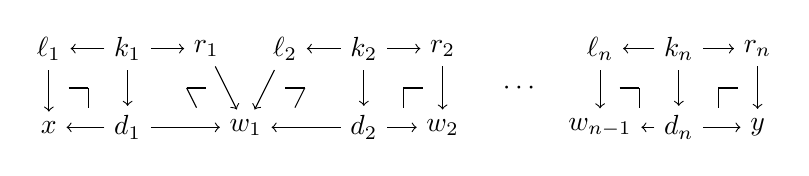
\begin{tikzpicture}
      \node (1t) at (0,1) {$ \ell_1 $};
      \node (2t) at (1,1) {$ k_1 $};
      \node (3t) at (2,1) {$ r_1 $};
      \node (4t) at (3,1) {$ \ell_2 $};
      \node (5t) at (4,1) {$ k_2 $};
      \node (6t) at (5,1) {$ r_2 $};
      \node (7t) at (7,1) {$ \ell_n $};
      \node (8t) at (8,1) {$ k_n $};
      \node (9t) at (9,1) {$ r_n $};
      \node (1b) at (0,0) {$ x $};
      \node (2b) at (1,0) {$ d_1 $};
      \node (3b) at (2.5,0) {$ w_1 $};
      \node (4b) at (4,0) {$ d_2 $};
      \node (5b) at (5,0) {$ w_2 $};
      \node (6b) at (7,0) {$ w_{n-1} $};
      \node (7b) at (8,0) {$ d_n $};
      \node (8b) at (9,0) {$ y $};
      \draw [->] (2t) to node [] {\scriptsize{$  $}} (1t);
      \draw [->] (2t) to node [] {\scriptsize{$  $}} (3t);
      \draw [->] (5t) to node [] {\scriptsize{$  $}} (4t);
      \draw [->] (5t) to node [] {\scriptsize{$  $}} (6t);
      \draw [->] (8t) to node [] {\scriptsize{$  $}} (7t);
      \draw [->] (8t) to node [] {\scriptsize{$  $}} (9t);
      \draw [->] (2b) to node [] {\scriptsize{$  $}} (1b);
      \draw [->] (2b) to node [] {\scriptsize{$  $}} (3b);
      \draw [->] (4b) to node [] {\scriptsize{$  $}} (3b);
      \draw [->] (4b) to node [] {\scriptsize{$  $}} (5b);
      \draw [->] (7b) to node [] {\scriptsize{$  $}} (6b);
      \draw [->] (7b) to node [] {\scriptsize{$  $}} (8b);
      \draw [->] (1t) to node [] {\scriptsize{$  $}} (1b);
      \draw [->] (2t) to node [] {\scriptsize{$  $}} (2b);
      \draw [->] (3t) to node [] {\scriptsize{$  $}} (3b);
      \draw [->] (4t) to node [] {\scriptsize{$  $}} (3b);
      \draw [->] (5t) to node [] {\scriptsize{$  $}} (4b);
      \draw [->] (6t) to node [] {\scriptsize{$  $}} (5b);
      \draw [->] (7t) to node [] {\scriptsize{$  $}} (6b);
      \draw [->] (8t) to node [] {\scriptsize{$  $}} (7b);
      \draw [->] (9t) to node [] {\scriptsize{$  $}} (8b);
      \node () at (6,0.5) {$ \dotsm $};
      \begin{scope}[shift={(0,0)}]
        % \draw [-] (0,0.25) to (0,0.5);
        \draw [-] (0.25,0.5) to node [] {} (0.5,0.5);
        \draw [-] (0.5,0.5) to node [] {} (0.5,0.25);
      \end{scope}
      \begin{scope}[shift={(1.75,0)}]
        \draw [-] (0.125,0.25) to (0,0.5);
        \draw [-] (0,0.5) to (0.25,0.5);
        % \draw [-] (0.5,0.5) to 5,0.25);
      \end{scope}
      \begin{scope}[shift={(2.75,0)}]
        % \draw [-] (0,0.25) to (0,0.5);
        \draw [-] (0.25,0.5) to node [] {} (0.5,0.5);
        \draw [-] (0.5,0.5) to node [] {} (0.375,0.25);
      \end{scope}
      \begin{scope}[shift={(4.5,0)}]
        \draw [-] (0,0.25) to (0,0.5);
        \draw [-] (0,0.5) to (0.25,0.5);
        % \draw [-] (0.5,0.5) to 5,0.25);
      \end{scope}
      \begin{scope}[shift={(7,0)}]
        % \draw [-] (0,0.25) to (0,0.5);
        \draw [-] (0.25,0.5) to node [] {} (0.5,0.5);
        \draw [-] (0.5,0.5) to node [] {} (0.5,0.25);
      \end{scope}
      \begin{scope}[shift={(8.5,0)}]
        \draw [-] (0,0.25) to (0,0.5);
        \draw [-] (0,0.5) to (0.25,0.5);
        % \draw [-] (0.5,0.5) to 5,0.25);
      \end{scope}     
    \end{tikzpicture}
  \]
  %
  and the derivation $ \deriv{x'}{y'} $ comes from a string
  of double pushout diagrams
  %
  \[
    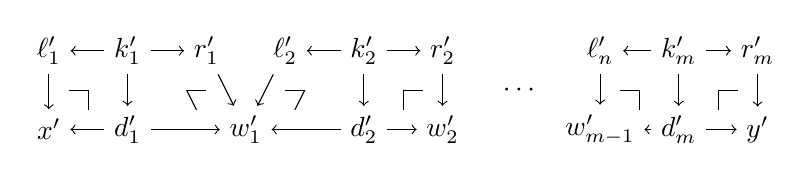
\begin{tikzpicture}
      \node (1t) at (0,1) {$ \ell'_1 $};
      \node (2t) at (1,1) {$ k'_1 $};
      \node (3t) at (2,1) {$ r'_1 $};
      \node (4t) at (3,1) {$ \ell'_2 $};
      \node (5t) at (4,1) {$ k'_2 $};
      \node (6t) at (5,1) {$ r'_2 $};
      \node (7t) at (7,1) {$ \ell'_n $};
      \node (8t) at (8,1) {$ k'_m $};
      \node (9t) at (9,1) {$ r'_m $};
      \node (1b) at (0,0) {$ x' $};
      \node (2b) at (1,0) {$ d'_1 $};
      \node (3b) at (2.5,0) {$ w'_1 $};
      \node (4b) at (4,0) {$ d'_2 $};
      \node (5b) at (5,0) {$ w'_2 $};
      \node (6b) at (7,0) {$ w'_{m-1} $};
      \node (7b) at (8,0) {$ d'_m $};
      \node (8b) at (9,0) {$ y' $};
      \draw [->] (2t) to node [] {\scriptsize{$  $}} (1t);
      \draw [->] (2t) to node [] {\scriptsize{$  $}} (3t);
      \draw [->] (5t) to node [] {\scriptsize{$  $}} (4t);
      \draw [->] (5t) to node [] {\scriptsize{$  $}} (6t);
      \draw [->] (8t) to node [] {\scriptsize{$  $}} (7t);
      \draw [->] (8t) to node [] {\scriptsize{$  $}} (9t);
      \draw [->] (2b) to node [] {\scriptsize{$  $}} (1b);
      \draw [->] (2b) to node [] {\scriptsize{$  $}} (3b);
      \draw [->] (4b) to node [] {\scriptsize{$  $}} (3b);
      \draw [->] (4b) to node [] {\scriptsize{$  $}} (5b);
      \draw [->] (7b) to node [] {\scriptsize{$  $}} (6b);
      \draw [->] (7b) to node [] {\scriptsize{$  $}} (8b);
      \draw [->] (1t) to node [] {\scriptsize{$  $}} (1b);
      \draw [->] (2t) to node [] {\scriptsize{$  $}} (2b);
      \draw [->] (3t) to node [] {\scriptsize{$  $}} (3b);
      \draw [->] (4t) to node [] {\scriptsize{$  $}} (3b);
      \draw [->] (5t) to node [] {\scriptsize{$  $}} (4b);
      \draw [->] (6t) to node [] {\scriptsize{$  $}} (5b);
      \draw [->] (7t) to node [] {\scriptsize{$  $}} (6b);
      \draw [->] (8t) to node [] {\scriptsize{$  $}} (7b);
      \draw [->] (9t) to node [] {\scriptsize{$  $}} (8b);
      \node () at (6,0.5) {$ \dotsm $};
      \begin{scope}[shift={(0,0)}]
        % \draw [-] (0,0.25) to (0,0.5);
        \draw [-] (0.25,0.5) to node [] {} (0.5,0.5);
        \draw [-] (0.5,0.5) to node [] {} (0.5,0.25);
      \end{scope}
      \begin{scope}[shift={(1.75,0)}]
        \draw [-] (0.125,0.25) to (0,0.5);
        \draw [-] (0,0.5) to (0.25,0.5);
        % \draw [-] (0.5,0.5) to 5,0.25);
      \end{scope}
      \begin{scope}[shift={(2.75,0)}]
        % \draw [-] (0,0.25) to (0,0.5);
        \draw [-] (0.25,0.5) to node [] {} (0.5,0.5);
        \draw [-] (0.5,0.5) to node [] {} (0.375,0.25);
      \end{scope}
      \begin{scope}[shift={(4.5,0)}]
        \draw [-] (0,0.25) to (0,0.5);
        \draw [-] (0,0.5) to (0.25,0.5);
        % \draw [-] (0.5,0.5) to 5,0.25);
      \end{scope}
      \begin{scope}[shift={(7,0)}]
        % \draw [-] (0,0.25) to (0,0.5);
        \draw [-] (0.25,0.5) to node [] {} (0.5,0.5);
        \draw [-] (0.5,0.5) to node [] {} (0.5,0.25);
      \end{scope}
      \begin{scope}[shift={(8.5,0)}]
        \draw [-] (0,0.25) to (0,0.5);
        \draw [-] (0,0.5) to (0.25,0.5);
        % \draw [-] (0.5,0.5) to 5,0.25);
      \end{scope}
    \end{tikzpicture}
  \]
  % 
  realize $ \deriv{x+x'}{y+y'} $  by concatenating
  to the end of first string with $ x' $ summed with the
  bottom row the second string with $ y $ summed on the
  bottom row.
\end{proof}

The main result ensures the possibility to study systems, as
represented by objects in a topos $ \X $, locally. To
reiterate, using structured cospans, we equip systems with
interfaces that allow us to connect them together. Another
way to view this is that we decompose a system into
sub-systems which are each studied then reconnected along
the interfaces that structured cospans provide. We discuss
the manner in which the main result does this below the
theorem, for which we need the following definition.

\begin{definition}
  Associate to a grammar $ ( \X , P ) $ the structured
  cospan grammar $ ( _{L}\StrCsp, P' ) $ where $ P' $
  contains
%
  \[
    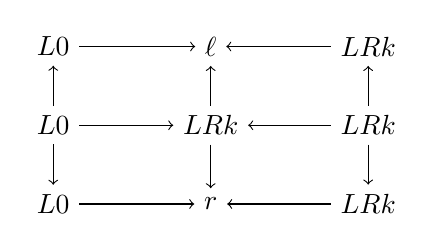
\begin{tikzpicture}
      \node (1) at (0,2) {$ L 0 $}; \node (2) at (2,2)
      {$ \ell $}; \node (3) at (4,2) {$ LRk
        $}; \node (4) at (0,1) {$ L 0
        $}; \node (5) at (2,1) {$ LRk
        $}; \node (6) at (4,1) {$ LRk
        $}; \node (7) at (0,0) {$ L 0
        $}; \node (8) at (2,0) {$ r
        $}; \node (9) at (4,0) {$ LRk
        $}; \draw [->] (1) to node [] {\scriptsize{$
          $}} (2); \draw [->] (3) to node []
      {\scriptsize{$
          $}} (2); \draw [->] (4) to node []
      {\scriptsize{$
          $}} (5); \draw [->] (6) to node []
      {\scriptsize{$
          $}} (5); \draw [->] (7) to node []
      {\scriptsize{$
          $}} (8); \draw [->] (9) to node []
      {\scriptsize{$
          $}} (8); \draw [->] (4) to node []
      {\scriptsize{$
          $}} (1); \draw [->] (4) to node []
      {\scriptsize{$
          $}} (7); \draw [->] (5) to node []
      {\scriptsize{$
          $}} (2); \draw [->] (5) to node []
      {\scriptsize{$
          $}} (8); \draw [->] (6) to node []
      {\scriptsize{$
          $}} (3); \draw [->] (6) to node []
      {\scriptsize{$ $}} (9);
    \end{tikzpicture}
  \]
% 
  for every rule $ LRk \to \ell \times r $ of $ P_{\flat} $.
\end{definition}

Before stating the theorem, we note that this is a
generalization of work by Gadducci and Heckle
\cite{Gadd_IndGraphTrans} and the structure of our proof is
an appropriate modification of theirs.

\begin{theorem} \label{thm:inductive-rewriting}
  Fix a geometric morphism $ L \dashv R \from \X \to \A $
  with monic counit. Let $ ( \X , P ) $ be a grammar such
  that for every $ \X $-object $ x $ in the apex of a
  production of $ P $, the Heyting algebra $ \Sub (x) $ is
  well-founded. Given $ g $, $ h \in \X $, then
  $ \deriv{g}{h} $ in the rewriting relation for a grammar
  $ ( \X , P ) $ if and only if there is a square
  %
  \[
    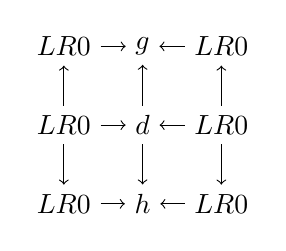
\begin{tikzpicture}
      \node (1t) at (0,2) {$ LR 0 $};
      \node (2t) at (1,2) {$ g $};
      \node (3t) at (2,2) {$ LR 0 $};
      \node (1m) at (0,1) {$ LR 0 $};
      \node (2m) at (1,1) {$ d $};
      \node (3m) at (2,1) {$ LR 0 $};
      \node (1b) at (0,0) {$ LR 0 $};
      \node (2b) at (1,0) {$ h $};
      \node (3b) at (2,0) {$ LR 0 $};
      \draw [->] (1t) to node [] {\scriptsize{$  $}} (2t);
      \draw [->] (3t) to node [] {\scriptsize{$  $}} (2t);
      \draw [->] (1m) to node [] {\scriptsize{$  $}} (2m);
      \draw [->] (3m) to node [] {\scriptsize{$  $}} (2m);
      \draw [->] (1b) to node [] {\scriptsize{$  $}} (2b);
      \draw [->] (3b) to node [] {\scriptsize{$  $}} (2b);
      \draw [->] (1m) to node [] {\scriptsize{$  $}} (1t);
      \draw [->] (1m) to node [] {\scriptsize{$  $}} (1b);
      \draw [->] (2m) to node [] {\scriptsize{$  $}} (2t);
      \draw [->] (2m) to node [] {\scriptsize{$  $}} (2b);
      \draw [->] (3m) to node [] {\scriptsize{$  $}} (3t);
      \draw [->] (3m) to node [] {\scriptsize{$  $}} (3b);
    \end{tikzpicture}
  \]
  % 
  in the double category $ \Lang ( _{L}\StrCsp , P' ) $.
\end{theorem}

\begin{proof}
  We show sufficiency by induction on the length of the
  derivation. If $ \dderiv{g}{h} $
  %
  \[
  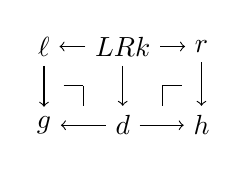
\begin{tikzpicture}
    \node (1t) at (0,1) {$ \ell $};
    \node (2t) at (1,1) {$ LRk $};
    \node (3t) at (2,1) {$ r $};
    \node (1b) at (0,0) {$ g $};
    \node (2b) at (1,0) {$ d $};
    \node (3b) at (2,0) {$ h $};
    \draw [->] (2t) to node [] {\scriptsize{$  $}} (1t);
    \draw [->] (2t) to node [] {\scriptsize{$  $}} (3t);
    \draw [->] (2b) to node [] {\scriptsize{$  $}} (1b);
    \draw [->] (2b) to node [] {\scriptsize{$  $}} (3b);
    \draw [->] (1t) to node [] {\scriptsize{$  $}} (1b);
    \draw [->] (2t) to node [] {\scriptsize{$  $}} (2b);
    \draw [->] (3t) to node [] {\scriptsize{$  $}} (3b);
       \begin{scope}[shift={(0,0)}]
        % \draw [-] (0,0.25) to (0,0.5);
        \draw [-] (0.25,0.5) to node [] {} (0.5,0.5);
        \draw [-] (0.5,0.5) to node [] {} (0.5,0.25);
      \end{scope}
      \begin{scope}[shift={(1.5,0)}]
        \draw [-] (0,0.25) to (0,0.5);
        \draw [-] (0,0.5) to (0.25,0.5);
        % \draw [-] (0.5,0.5) to 5,0.25);
      \end{scope}
  \end{tikzpicture}
  \]
  % 
  the desired square is the horizontal composition of
  %
  \[
    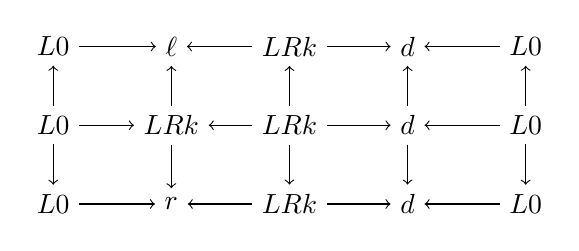
\begin{tikzpicture}
    \begin{scope}
      \node (1t) at (0,2) {$ L0 $};
      \node (2t) at (1.5,2) {$ \ell $};
      \node (3t) at (3,2) {$ LRk $};
      \node (4t) at (4.5,2) {$ d $};
      \node (5t) at (6,2) {$ L0 $};
      \node (1m) at (0,1) {$ L 0 $};
      \node (2m) at (1.5,1) {$ LRk $};
      \node (3m) at (3,1) {$ LRk $};
      \node (4m) at (4.5,1) {$ d $};
      \node (5m) at (6,1) {$ L 0 $};
      \node (1b) at (0,0) {$ L 0 $};
      \node (2b) at (1.5,0) {$ r $};
      \node (3b) at (3,0) {$ LRk $};
      \node (4b) at (4.5,0) {$ d $};
      \node (5b) at (6,0) {$ L 0 $};
      \draw [->] (1t) to node [] {\scriptsize{$  $}} (2t);
      \draw [->] (3t) to node [] {\scriptsize{$  $}} (2t);
      \draw [->] (3t) to node [] {\scriptsize{$  $}} (4t);
      \draw [->] (5t) to node [] {\scriptsize{$  $}} (4t);
      \draw [->] (1m) to node [] {\scriptsize{$  $}} (2m);
      \draw [->] (3m) to node [] {\scriptsize{$  $}} (2m);
      \draw [->] (3m) to node [] {\scriptsize{$  $}} (4m);
      \draw [->] (5m) to node [] {\scriptsize{$  $}} (4m);
      \draw [->] (1b) to node [] {\scriptsize{$  $}} (2b);
      \draw [->] (3b) to node [] {\scriptsize{$  $}} (2b);
      \draw [->] (3b) to node [] {\scriptsize{$  $}} (4b);
      \draw [->] (5b) to node [] {\scriptsize{$  $}} (4b);
      \draw [->] (1m) to node [] {\scriptsize{$  $}} (1t);
      \draw [->] (1m) to node [] {\scriptsize{$  $}} (1b);
      \draw [->] (2m) to node [] {\scriptsize{$  $}} (2t);
      \draw [->] (2m) to node [] {\scriptsize{$  $}} (2b);
      \draw [->] (3m) to node [] {\scriptsize{$  $}} (3t);
      \draw [->] (3m) to node [] {\scriptsize{$  $}} (3b);
      \draw [->] (4m) to node [] {\scriptsize{$  $}} (4t);
      \draw [->] (4m) to node [] {\scriptsize{$  $}} (4b);
      \draw [->] (5m) to node [] {\scriptsize{$  $}} (5t);
      \draw [->] (5m) to node [] {\scriptsize{$  $}} (5b);
    \end{scope}
    \end{tikzpicture}
  \]
  %
  The left square is a generator and the right square is the
  identity on the horizontal arrow $ LRk + L \empty \to d
  $. The square for a derivation
  $ \dderiv{\deriv{g}{h}}{j} $ is the vertical composition
  of
  %
  \[
    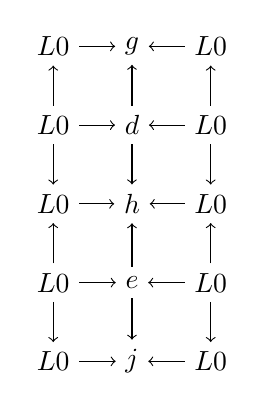
\begin{tikzpicture}
      \node (1t) at (0,4) {$ L 0 $};
      \node (2t) at (1,4) {$ g $};
      \node (3t) at (2,4) {$ L 0 $};
      \node (1m) at (0,3) {$ L 0 $};
      \node (2m) at (1,3) {$ d $};
      \node (3m) at (2,3) {$ L 0 $};
      \node (1b) at (0,2) {$ L 0 $};
      \node (2b) at (1,2) {$ h $};
      \node (3b) at (2,2) {$ L 0 $};
      \node (1bb) at (0,1) {$ L 0 $};
      \node (2bb) at (1,1) {$ e $};
      \node (3bb) at (2,1) {$ L 0 $};
      \node (1bbb) at (0,0) {$ L 0 $};
      \node (2bbb) at (1,0) {$ j $};
      \node (3bbb) at (2,0) {$ L 0 $};
      \draw [->] (1t) to node [] {\scriptsize{$  $}} (2t);
      \draw [->] (3t) to node [] {\scriptsize{$  $}} (2t);
      \draw [->] (1m) to node [] {\scriptsize{$  $}} (2m);
      \draw [->] (3m) to node [] {\scriptsize{$  $}} (2m);
      \draw [->] (1b) to node [] {\scriptsize{$  $}} (2b);
      \draw [->] (3b) to node [] {\scriptsize{$  $}} (2b);
      \draw [->] (1m) to node [] {\scriptsize{$  $}} (1t);
      \draw [->] (1m) to node [] {\scriptsize{$  $}} (1b);
      \draw [->] (2m) to node [] {\scriptsize{$  $}} (2t);
      \draw [->] (2m) to node [] {\scriptsize{$  $}} (2b);
      \draw [->] (3m) to node [] {\scriptsize{$  $}} (3t);
      \draw [->] (3m) to node [] {\scriptsize{$  $}} (3b);
      \draw [->] (1bb) to node [] {\scriptsize{$  $}} (2bb);
      \draw [->] (3bb) to node [] {\scriptsize{$  $}} (2bb);
      \draw [->] (1bbb) to node [] {\scriptsize{$  $}} (2bbb);
      \draw [->] (3bbb) to node [] {\scriptsize{$  $}} (2bbb);
      \draw [->] (1bb) to node [] {\scriptsize{$  $}} (1b);
      \draw [->] (1bb) to node [] {\scriptsize{$  $}} (1bbb);
      \draw [->] (2bb) to node [] {\scriptsize{$  $}} (2b);
      \draw [->] (2bb) to node [] {\scriptsize{$  $}} (2bbb);
      \draw [->] (3bb) to node [] {\scriptsize{$  $}} (3b);
      \draw [->] (3bb) to node [] {\scriptsize{$  $}} (3bbb);
    \end{tikzpicture}
  \]
  %
  The top square is from $ \deriv{g}{h} $ and the second
  from $ \dderiv{h}{j} $.

  Conversely, proceed by structural induction on the
  generating squares of $ \Lang ( _{L}\StrCsp , P' ) $.  It
  suffices to show that the rewrite relation is preserved by
  vertical and composition by a generating square.  Suppose
  we have a square
  %
  \[
    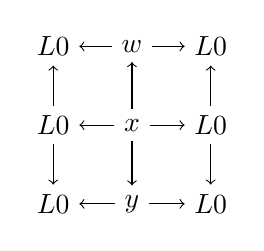
\begin{tikzpicture}
      \node (1t) at (0,2) {$ L 0 $};
      \node (2t) at (1,2) {$ w $};
      \node (3t) at (2,2) {$ L 0 $};
      \node (1m) at (0,1) {$ L 0 $};
      \node (2m) at (1,1) {$ x $};
      \node (3m) at (2,1) {$ L 0 $};
      \node (1b) at (0,0) {$ L 0 $};
      \node (2b) at (1,0) {$ y $};
      \node (3b) at (2,0) {$ L 0 $};
      \draw [->] (2t) to node [] {\scriptsize{$  $}} (1t);
      \draw [->] (2t) to node [] {\scriptsize{$  $}} (3t);
      \draw [->] (2m) to node [] {\scriptsize{$  $}} (1m);
      \draw [->] (2m) to node [] {\scriptsize{$  $}} (3m);
      \draw [->] (2b) to node [] {\scriptsize{$  $}} (1b);
      \draw [->] (2b) to node [] {\scriptsize{$  $}} (3b);
      \draw [->] (1m) to node [] {\scriptsize{$  $}} (1t);
      \draw [->] (2m) to node [] {\scriptsize{$  $}} (2t);
      \draw [->] (3m) to node [] {\scriptsize{$  $}} (3t);
      \draw [->] (1m) to node [] {\scriptsize{$  $}} (1b);
      \draw [->] (2m) to node [] {\scriptsize{$  $}} (2b);
      \draw [->] (3m) to node [] {\scriptsize{$  $}} (3b);
    \end{tikzpicture}
  \]
  % 
  corresponding to a derivation $ \deriv{w}{y} $. Composing
  this vertically with a generating square, which must have
  form
  %
  \[
    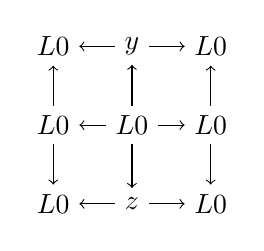
\begin{tikzpicture}
      \node (1t) at (0,2) {$ L 0 $};
      \node (2t) at (1,2) {$ y $};
      \node (3t) at (2,2) {$ L 0 $};
      \node (1m) at (0,1) {$ L 0 $};
      \node (2m) at (1,1) {$ L 0 $};
      \node (3m) at (2,1) {$ L 0 $};
      \node (1b) at (0,0) {$ L 0 $};
      \node (2b) at (1,0) {$ z $};
      \node (3b) at (2,0) {$ L 0 $};
      \draw [->] (2t) to node [] {\scriptsize{$  $}} (1t);
      \draw [->] (2t) to node [] {\scriptsize{$  $}} (3t);
      \draw [->] (2m) to node [] {\scriptsize{$  $}} (1m);
      \draw [->] (2m) to node [] {\scriptsize{$  $}} (3m);
      \draw [->] (2b) to node [] {\scriptsize{$  $}} (1b);
      \draw [->] (2b) to node [] {\scriptsize{$  $}} (3b);
      \draw [->] (1m) to node [] {\scriptsize{$  $}} (1t);
      \draw [->] (2m) to node [] {\scriptsize{$  $}} (2t);
      \draw [->] (3m) to node [] {\scriptsize{$  $}} (3t);
      \draw [->] (1m) to node [] {\scriptsize{$  $}} (1b);
      \draw [->] (2m) to node [] {\scriptsize{$  $}} (2b);
      \draw [->] (3m) to node [] {\scriptsize{$  $}} (3b);
    \end{tikzpicture}
  \]
  %
  corresponding to a production $ 0 \to y + z $ gives
  %
  \[
    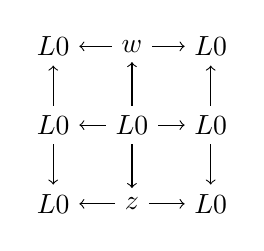
\begin{tikzpicture}
      \node (1t) at (0,2) {$ L 0 $};
      \node (2t) at (1,2) {$ w $};
      \node (3t) at (2,2) {$ L 0 $};
      \node (1m) at (0,1) {$ L 0 $};
      \node (2m) at (1,1) {$ L 0 $};
      \node (3m) at (2,1) {$ L 0 $};
      \node (1b) at (0,0) {$ L 0 $};
      \node (2b) at (1,0) {$ z $};
      \node (3b) at (2,0) {$ L 0 $};
      \draw [->] (2t) to node [] {\scriptsize{$  $}} (1t);
      \draw [->] (2t) to node [] {\scriptsize{$  $}} (3t);
      \draw [->] (2m) to node [] {\scriptsize{$  $}} (1m);
      \draw [->] (2m) to node [] {\scriptsize{$  $}} (3m);
      \draw [->] (2b) to node [] {\scriptsize{$  $}} (1b);
      \draw [->] (2b) to node [] {\scriptsize{$  $}} (3b);
      \draw [->] (1m) to node [] {\scriptsize{$  $}} (1t);
      \draw [->] (2m) to node [] {\scriptsize{$  $}} (2t);
      \draw [->] (3m) to node [] {\scriptsize{$  $}} (3t);
      \draw [->] (1m) to node [] {\scriptsize{$  $}} (1b);
      \draw [->] (2m) to node [] {\scriptsize{$  $}} (2b);
      \draw [->] (3m) to node [] {\scriptsize{$  $}} (3b);
    \end{tikzpicture}
  \]
  %
  which corresponds to a derivation
  $ \dderiv{\deriv{w}{y}}{z} $.  Composing horizontally with
  a generating square
  %
  \[
    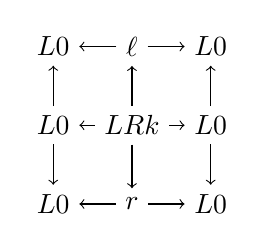
\begin{tikzpicture}
      \node (1t) at (0,2) {$ L 0 $};
      \node (2t) at (1,2) {$ \ell $};
      \node (3t) at (2,2) {$ L 0 $};
      \node (1m) at (0,1) {$ L 0 $};
      \node (2m) at (1,1) {$ LRk $};
      \node (3m) at (2,1) {$ L 0 $};
      \node (1b) at (0,0) {$ L 0 $};
      \node (2b) at (1,0) {$ r $};
      \node (3b) at (2,0) {$ L 0 $};
      \draw [->] (2t) to node [] {\scriptsize{$  $}} (1t);
      \draw [->] (2t) to node [] {\scriptsize{$  $}} (3t);
      \draw [->] (2m) to node [] {\scriptsize{$  $}} (1m);
      \draw [->] (2m) to node [] {\scriptsize{$  $}} (3m);
      \draw [->] (2b) to node [] {\scriptsize{$  $}} (1b);
      \draw [->] (2b) to node [] {\scriptsize{$  $}} (3b);
      \draw [->] (1m) to node [] {\scriptsize{$  $}} (1t);
      \draw [->] (2m) to node [] {\scriptsize{$  $}} (2t);
      \draw [->] (3m) to node [] {\scriptsize{$  $}} (3t);
      \draw [->] (1m) to node [] {\scriptsize{$  $}} (1b);
      \draw [->] (2m) to node [] {\scriptsize{$  $}} (2b);
      \draw [->] (3m) to node [] {\scriptsize{$  $}} (3b);
    \end{tikzpicture}
  \]
  %
  corresponding with a production $ LRk \to \ell + r $
  results in the square
  %
  \[
    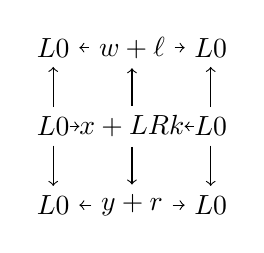
\begin{tikzpicture}
      \node (1t) at (0,2) {$ L 0 $};
      \node (2t) at (1,2) {$ w + \ell $};
      \node (3t) at (2,2) {$ L 0 $};
      \node (1m) at (0,1) {$ L 0 $};
      \node (2m) at (1,1) {$ x + LRk $};
      \node (3m) at (2,1) {$ L 0 $};
      \node (1b) at (0,0) {$ L 0 $};
      \node (2b) at (1,0) {$ y + r $};
      \node (3b) at (2,0) {$ L 0 $};
      \draw [->] (2t) to node [] {\scriptsize{$  $}} (1t);
      \draw [->] (2t) to node [] {\scriptsize{$  $}} (3t);
      \draw [->] (2m) to node [] {\scriptsize{$  $}} (1m);
      \draw [->] (2m) to node [] {\scriptsize{$  $}} (3m);
      \draw [->] (2b) to node [] {\scriptsize{$  $}} (1b);
      \draw [->] (2b) to node [] {\scriptsize{$  $}} (3b);
      \draw [->] (1m) to node [] {\scriptsize{$  $}} (1t);
      \draw [->] (2m) to node [] {\scriptsize{$  $}} (2t);
      \draw [->] (3m) to node [] {\scriptsize{$  $}} (3t);
      \draw [->] (1m) to node [] {\scriptsize{$  $}} (1b);
      \draw [->] (2m) to node [] {\scriptsize{$  $}} (2b);
      \draw [->] (3m) to node [] {\scriptsize{$  $}} (3b);
    \end{tikzpicture}
  \]
  %
  But $ \deriv{w+\ell}{y+r} $ as seen in Lemma
  \ref{thm:rewrite-rel-is-additive}. 

\end{proof}

With this result, we have completely described the rewrite
relation for a grammar $ ( \X , P ) $ with squares in
$ \Lang ( _{L}\StrCsp, P' ) $ framed by the initial
object of $ \X $.  These squares are rewrites of a closed
system in the sense that the interface is empty.  We can
instead begin with a closed system $ x $ in $ \X $ as
represented by a horizontal arrow $ \csp{L0}{x}{L0} $ in
$ \Lang ( _{L}\StrCsp , P' ) $ and decompose it into a
composite of sub-systems, that is a sequence of composable
horizontal arrows
%
\[
  L0 \to x_1 \gets La_1 \to x_2 \gets La_2 \dotsm La_{n-1} \to x_n
  \gets L0
\]
%y
Rewriting can be performed on each of these sub-systems
%
\[
  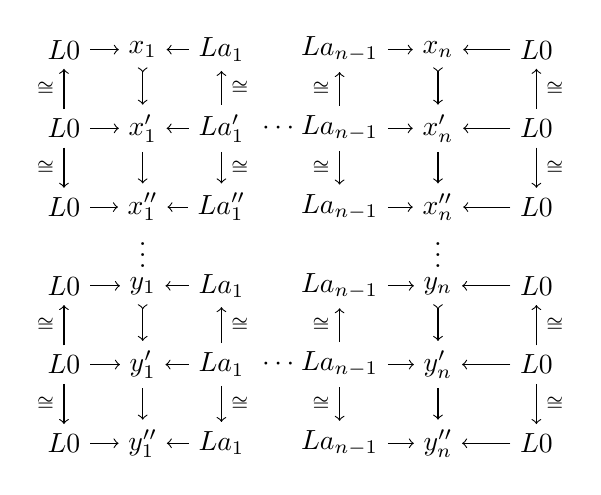
\begin{tikzpicture}
    \begin{scope}[shift={(0,3)}]
      \node (1) at (0,2) {$ L0 $};
      \node (2) at (1,2) {$ x_1 $};
      \node (3) at (2,2) {$ La_1 $};
      \node (4) at (0,1) {$ L0 $};
      \node (5) at (1,1) {$ x'_1 $};
      \node (6) at (2,1) {$ La'_1 $};
      \node (7) at (0,0) {$ L0 $};
      \node (8) at (1,0) {$ x''_1 $};
      \node (9) at (2,0) {$ La''_1 $};
      \draw [->] (1) to node [] {\scriptsize{$  $}} (2);
      \draw [->] (3) to node [] {\scriptsize{$  $}} (2);
      \draw [->] (4) to node [] {\scriptsize{$  $}} (5);
      \draw [->] (6) to node [] {\scriptsize{$  $}} (5);
      \draw [->] (7) to node [] {\scriptsize{$  $}} (8);
      \draw [->] (9) to node [] {\scriptsize{$  $}} (8);
      \draw [->] (4) to node [left] {\scriptsize{$ \cong $}} (1);
      \draw [->] (4) to node [left] {\scriptsize{$ \cong $}} (7);
      \draw [>->] (2) to node [] {\scriptsize{$  $}} (5);
      \draw [->] (5) to node [] {\scriptsize{$  $}} (8);
      \draw [->] (6) to node [right] {\scriptsize{$ \cong  $}} (3);
      \draw [->] (6) to node [right] {\scriptsize{$ \cong $}} (9);
    \end{scope}
    %
    \begin{scope}[shift={(3.5,3)}]
      \node (1) at (0,2) {$ La_{n-1} $};
      \node (2) at (1.25,2) {$ x_n $};
      \node (3) at (2.5,2) {$ L0 $};
      \node (4) at (0,1) {$ La_{n-1} $};
      \node (5) at (1.25,1) {$ x'_n $};
      \node (6) at (2.5,1) {$ L0 $};
      \node (7) at (0,0) {$ La_{n-1} $};
      \node (8) at (1.25,0) {$ x''_n $};
      \node (9) at (2.5,0) {$ L0 $};
       \draw [->] (1) to node [] {\scriptsize{$  $}} (2);
      \draw [->] (3) to node [] {\scriptsize{$  $}} (2);
      \draw [->] (4) to node [] {\scriptsize{$  $}} (5);
      \draw [->] (6) to node [] {\scriptsize{$  $}} (5);
      \draw [->] (7) to node [] {\scriptsize{$  $}} (8);
      \draw [->] (9) to node [] {\scriptsize{$  $}} (8);
      \draw [->] (4) to node [left] {\scriptsize{$ \cong $}} (1);
      \draw [->] (4) to node [left] {\scriptsize{$ \cong $}} (7);
      \draw [>->] (2) to node [] {\scriptsize{$  $}} (5);
      \draw [->] (5) to node [] {\scriptsize{$  $}} (8);
      \draw [->] (6) to node [right] {\scriptsize{$ \cong  $}} (3);
      \draw [->] (6) to node [right] {\scriptsize{$ \cong $}} (9);
    \end{scope}
    %
    \begin{scope}
      \node (1) at (0,2) {$ L0 $};
      \node (2) at (1,2) {$ y_1 $};
      \node (3) at (2,2) {$ La_1 $};
      \node (4) at (0,1) {$ L0 $};
      \node (5) at (1,1) {$ y'_1 $};
      \node (6) at (2,1) {$ La_1 $};
      \node (7) at (0,0) {$ L0 $};
      \node (8) at (1,0) {$ y''_1 $};
      \node (9) at (2,0) {$ La_1 $};
       \draw [->] (1) to node [] {\scriptsize{$  $}} (2);
      \draw [->] (3) to node [] {\scriptsize{$  $}} (2);
      \draw [->] (4) to node [] {\scriptsize{$  $}} (5);
      \draw [->] (6) to node [] {\scriptsize{$  $}} (5);
      \draw [->] (7) to node [] {\scriptsize{$  $}} (8);
      \draw [->] (9) to node [] {\scriptsize{$  $}} (8);
      \draw [->] (4) to node [left] {\scriptsize{$ \cong $}} (1);
      \draw [->] (4) to node [left] {\scriptsize{$ \cong $}} (7);
      \draw [>->] (2) to node [] {\scriptsize{$  $}} (5);
      \draw [->] (5) to node [] {\scriptsize{$  $}} (8);
      \draw [->] (6) to node [right] {\scriptsize{$ \cong  $}} (3);
      \draw [->] (6) to node [right] {\scriptsize{$ \cong $}} (9);
    \end{scope}
    %
    \begin{scope}[shift={(3.5,0)}]
      \node (1) at (0,2) {$ La_{n-1} $};
      \node (2) at (1.25,2) {$ y_n $};
      \node (3) at (2.5,2) {$ L0 $};
      \node (4) at (0,1) {$ La_{n-1} $};
      \node (5) at (1.25,1) {$ y'_n $};
      \node (6) at (2.5,1) {$ L0 $};
      \node (7) at (0,0) {$ La_{n-1} $};
      \node (8) at (1.25,0) {$y''_n $};
      \node (9) at (2.5,0) {$ L0 $};
       \draw [->] (1) to node [] {\scriptsize{$  $}} (2);
      \draw [->] (3) to node [] {\scriptsize{$  $}} (2);
      \draw [->] (4) to node [] {\scriptsize{$  $}} (5);
      \draw [->] (6) to node [] {\scriptsize{$  $}} (5);
      \draw [->] (7) to node [] {\scriptsize{$  $}} (8);
      \draw [->] (9) to node [] {\scriptsize{$  $}} (8);
      \draw [->] (4) to node [left] {\scriptsize{$ \cong $}} (1);
      \draw [->] (4) to node [left] {\scriptsize{$ \cong $}} (7);
      \draw [>->] (2) to node [] {\scriptsize{$  $}} (5);
      \draw [->] (5) to node [] {\scriptsize{$  $}} (8);
      \draw [->] (6) to node [right] {\scriptsize{$ \cong  $}} (3);
      \draw [->] (6) to node [right] {\scriptsize{$ \cong $}} (9);
    \end{scope}
    %
    \node () at (2.75,4) {$ \dotsm $};
    \node () at (1,2.5) {$ \vdots $};
    \node () at (2.75,1) {$ \dotsm $};
    \node () at (4.75,2.5) {$ \vdots $};
  \end{tikzpicture}
\]
%
The composite of these squares is a rewriting of the
original system.

% ~~~~~~~~~~~~~~~~~~~~~~~~~~~~~~~~~~~~~~~~
% 
% ~~~~~~~~~~~ bibliography ~~~~~~~~~~~~~~~
% 
% ~~~~~~~~~~~~~~~~~~~~~~~~~~~~~~~~~~~~~~~~

\begin{thebibliography}{99}
  % use APA style
  % \bibitem{1st-citation}

\bibitem{StrCsp} J.~Baez, K.~Courser. Structured
  cospans. \emph{In preparation}.

% \bibitem{NetMods} J.~Baez, J.~Foley, J.~Moeller,
%   B.~Pollard. Network Models. \emph{arXiv preprint}
%   \href{https://arxiv.org/abs/1711.00037}{arXiv:1711.00037}.
%   2017.

\bibitem{PassiveNets} J.~Baez, B.~Fong. A compositional
  framework for passive linear networks. \emph{Theory Appl.\
    Categ.} 33, No.\ 38, 1158--1222. 2018

\bibitem{MrkvProc} J.~Baez, B.~Fong, B.~Pollard. A
  compositional framework for Markov
  processes. \emph{J.~Math.~Phys.} 57, No.~3: 033301. 2016.
  
\bibitem{RxNets} J.~Baez, B.~Pollard. A compositional
  framework for reaction networks. \emph{Rev. Math. Phys.}
  29, No.~9, 1750028. 2017.

\bibitem{OpenPetri} J.~Baez, J.~Master. Open Petri
  nets. \emph{arXiv preprint}
  \href{https://arxiv.org/abs/1808.05414}{arXiv:1808.05414}. 2018.
  
\bibitem{Chomsky} N.~Chomsky. On certain formal properties
  of grammars.  \emph{Inf.~Control}. No.~2. 137-167. 1959.
  
\bibitem{Cic_SpCsp} D.\ Cicala. Spans of
  cospans. \emph{Theory Appl.\ Categ.} 33, No.\ 6,
  131--147. 2018.

\bibitem{CicCour_SpCspTopos} D.\ Cicala, K.\
  Courser. Spans of cospans in a topos. \emph{Theory Appl.\
    Categ.} 33, No.\ 1, 1--22. 2018.

\bibitem{DixKiss_OpenGraphs} L.\ Dixon, A.\
  Kissinger. Open-graphs and monoidal theories. \emph{Math.\
    Structures Comput.\ Sci.}, \textbf{23}, No.\ 2,
  308--359. 2013.

\bibitem{Ehrig_GraphGram} H.\ Ehrig, M.\ Pfender, H.J.\
  Schneider. Graph-grammars: An algebraic approach. In
  \emph{Switching and Automata Theory, 1973. SWAT'08. IEEE
    Conference Record of 14th Annual Symposium on},
  167--180. IEEE. 1973.
  
\bibitem{DecorCsp} B.\ Fong. Decorated cospans. \emph{Theory
    Appl.\ Categ.} 30, Paper No.\ 33, 1096--1120. 2015.
          
\bibitem{Gadd_IndGraphTrans} F.\ Gadducci, R.\ Heckel. An
  inductive view of graph transformation.\emph{International
    Workshop on Algebraic Development
    Techniques}. 223--237. Springer. 1998.

% \bibitem{DblPushoutRevis} A.~Habel, J.~M\:{u}ller,
%   D.~Plump. Double-pushout graph transformation
%   revisited. \emph{Math. Structures Comput. Sci.}
%   11. No.~5. 637--688. 2001).
  
\bibitem{LackSobo_Adhesive} S.\ Lack, P.\
  Soboci\'{n}ski. Adhesive categories. In
  \emph{International Conference on Foundations of Software
    Science and Computation Structures},
  273--288. Springer. 2004.

\bibitem{LackSobo_ToposIsAdh} S.~Lack,
  P.~Soboci\'{n}ski. Toposes are
  adhesive. \emph{International Conference on Graph
    Transformation}. Springer. 2006.

\bibitem{ShulDblCat} M.~Shulman. Constructing symmetric
  monoidal bicategories. \emph{arXiv preprint}
  \href{https://arxiv.org/abs/1004.0993}{arXiv:1004.0993}
  2010.
  
\bibitem{Wraith_ArtinGlue} G.\ Wraith. Artin
  gluing. \emph{J.\ Pure Appl.\ Algebra} \textbf{4},
  345--348. 1974.

\end{thebibliography}

\end{document}
